% Document: Bachelor Thesis: Minimal Problem Solver Generator
% Author: Pavel Trutman

\documentclass[msc]{cmpthesis}
\usepackage[czech,english]{babel}
\usepackage[utf8]{inputenc}
\usepackage{indentfirst}
\usepackage{enumitem}
\usepackage{textcomp}
\usepackage{algorithm}
\usepackage{algpseudocode}
\usepackage{listings}
\usepackage{amsmath}
\usepackage{amssymb}
\usepackage{amsthm}
\usepackage{forloop}

\usepackage{subcaption}
\usepackage{pdflscape}
\usepackage{multirow}
\usepackage{dirtree}

% for better verbatim environment
\usepackage{fancyvrb}

% to inlucude pdf pages
\usepackage{pdfpages}

% list of symbols and abbreviations
\usepackage[acronym,nonumberlist,style=long,sort=def]{glossaries}
\setlength{\glsdescwidth}{0.7\linewidth}
\setlength{\glspagelistwidth}{0.3\linewidth}
\renewcommand*{\glsgroupskip}{}
\newcommand{\Acronym}[2]{\newacronym{#1}{#1}{#2}}
\Acronym{cl$(S)$}{Closure of the set $S$}
\Acronym{dom $f$}{Domain of the function $f$}
\Acronym{Dom $f$}{cl(dom $f$)}
\Acronym{int $S$}{Interior of the set $S$}
\newacronym{P}{$\mathcal{P}^n$}{Cone of positive semidefinite $n\times n$ matrices}
\newacronym{S}{$\mathcal{S}^n$}{Space of $n\times n$ real symmetric matrices}
\Acronym{tr$(A)$}{Trace of the matrix $A$}
\newacronym{i-th element of x}{$x^{(i)}$}{$i$-th element of the vector $x$}

\makeglossaries

% algorithmic macros and settings
\newcounter{counter}
\renewcommand{\algorithmicrequire}{\textbf{Input:}}
\renewcommand{\algorithmicensure}{\textbf{Output:}}
\algdef{S}[IF]{IfML}[1]{\algorithmicif\ #1}
\newcommand{\StatexIndent}[1][1]{
  \Statex\forloop{counter}{0}{\value{counter} < #1}{\hskip\algorithmicindent\hskip-0.25em}
}
\renewcommand{\thealgorithm}{\arabic{chapter}.\arabic{algorithm}}
\DeclareCaptionFormat{algorithm}{#1#2#3}
\captionsetup[algorithm]{format=algorithm, labelsep=period}

% listings settings
\makeatletter
\def\lst@numbersymbol{}
\lst@Key{numbersymbol}{}{\def\lst@numbersymbol{#1}}
\lst@Key{numbers}{none}{%
  \let\lst@PlaceNumber\@empty
  \lstKV@SwitchCases{#1}%
  {none&\\%
  left&\def\lst@PlaceNumber{\llap{\normalfont
      \lst@numberstyle{\thelstnumber\lst@numbersymbol}\kern\lst@numbersep}}\\%
  right&\def\lst@PlaceNumber{\rlap{\normalfont
      \kern\linewidth \kern\lst@numbersep
      \lst@numberstyle{\lst@numbersymbol\thelstnumber}}}%
  }{\PackageError{Listings}{Numbers #1 unknown}\@ehc}}
\def\lst@labellis{}
\lst@Key{labellis}{}{\def\lst@label{listing:#1}}
\makeatother
\lstset{basicstyle=\normalfont\ttfamily,
  columns=fixed,
  basewidth=0.5em,
  showstringspaces=false,
  breaklines=true,
  commentstyle=\color{blue},
  keywordstyle=\color{red},
  numbers=left,
  numberstyle=\footnotesize\normalfont,
  numbersymbol=:,
  captionpos=t,
  frame=top,
  frame=bottom,
  xleftmargin=25pt,
  framexleftmargin=25pt,
}
\DeclareCaptionFormat{listing}{\rule{\dimexpr\textwidth\relax}{1pt}\vskip-3pt\hspace{-10pt}#1#2#3}
\captionsetup[lstlisting]{format=listing, singlelinecheck=false, labelsep=period}
\renewcommand\lstlistlistingname{List of Listings}

% hyphen - as active for hyphenation breaks cline command
\usepackage{regexpatch}
\makeatletter
% Change the `-` delimiter to an active character
\xpatchparametertext\@@@cmidrule{-}{\cA-}{}{}
\xpatchparametertext\@cline{-}{\cA-}{}{}
\makeatother

\startThesisInfo
\title{Semidefinite Programming for Geometric Problems in Computer Vision}
\author{Pavel Trutman}
\CMPAdvisor{Ing. Tom\'a\v s Pajdla, PhD.}
\CMPReportNo{}
\CMPAcknowledgement{\centering }

\CMPEmail{pavel.trutman@fel.cvut.cz}
\CMPDocumentURL{http://cmp.felk.cvut.cz/~trutmpav/master-thesis/thesis/thesis.pdf}
\stopThesisInfo

% ============================== your definitions (abbreviations etc.)
\newcommand{\eqB}{\begin{eqnarray}}
\newcommand{\eqE}{\end{eqnarray}}
\newcommand{\bmB}{\begin{bmatrix}}
\newcommand{\bmE}{\end{bmatrix}}
\newcommand{\ind}[1]{\ensuremath{^{(#1)}}}
\newcommand{\labeldef}[1]{\label{definition:#1}}
\newcommand{\refdef}[1]{Definition~\ref{definition:#1}}
\newcommand{\labelcol}[1]{\label{corollary:#1}}
\newcommand{\refcol}[1]{Corollary~\ref{corollary:#1}}
\newcommand{\labelthe}[1]{\label{theorem:#1}}
\newcommand{\refthe}[1]{Theorem~\ref{theorem:#1}}
\newcommand{\labelex}[1]{\label{example:#1}}
\newcommand{\refex}[1]{Example~\ref{example:#1}}
\newcommand{\labeleq}[1]{\label{equation:#1}}
\newcommand{\refeq}[1]{Equation~(\ref{equation:#1})}
\newcommand{\refeqb}[1]{(\ref{equation:#1})}
\newcommand{\labelalg}[1]{\label{algorithm:#1}}
\newcommand{\refalg}[1]{Algorithm~\ref{algorithm:#1}}
\newcommand{\labelalgline}[1]{\label{algorithm:line:#1}}
\newcommand{\refalgline}[1]{\ref{algorithm:line:#1}}
\newcommand{\labelfig}[1]{\label{figure:#1}}
\newcommand{\reffig}[1]{Figure~\ref{figure:#1}}
\newcommand{\labeltab}[1]{\label{table:#1}}
\newcommand{\reftab}[1]{Table~\ref{table:#1}}
\newcommand{\labelsec}[1]{\label{section:#1}}
\newcommand{\refsec}[1]{Section~\ref{section:#1}}
\newcommand{\labelcha}[1]{\label{chapter:#1}}
\newcommand{\refcha}[1]{Chapter~\ref{chapter:#1}}
\newcommand{\reflis}[1]{Listing~\ref{listing:#1}}
\newtheoremstyle{definitionStyle}
  {}
  {}
  {}
  {}
  {\bfseries}
  {.}
  { }
  {\thmname{#1}\thmnumber{ #2}\thmnote{ (#3)}}
\theoremstyle{definitionStyle}
\newtheorem{definition}{Definition}[chapter]
\newtheorem{theorem}{Theorem}[chapter]
\newtheorem{example}{Example}[chapter]
\newtheorem{corollary}{Corollary}[chapter]
\newcommand{\R}{\mathbb{R}}
\newcommand{\N}{\mathbb{N}}
\newcommand{\C}{\mathbb{C}}
\newcommand{\Z}{\mathbb{Z}}
\newcommand{\Sym}{\mathcal{S}}
\newcommand{\PSDCone}{\mathcal{P}}
\newcommand{\Iden}[1]{\ensuremath{\mathcal{I}^{#1}}}
\newcommand{\Ideal}{\mathcal{I}}
\newcommand{\Base}{\mathcal{B}}
\newcommand{\NF}{\mathcal{N}}
\newcommand{\MM}{\mathcal{X}}
\DeclareMathOperator{\rank}{rank}
\DeclareMathOperator{\dom}{dom}
\DeclareMathOperator{\Dom}{Dom}
\DeclareMathOperator{\cl}{cl}
\DeclareMathOperator{\inter}{int}
\DeclareMathOperator{\tr}{tr}
\DeclareMathOperator{\diag}{diag}

\def\CC{{C\nolinebreak[4]\hspace{-.05em}\raisebox{.4ex}{\tiny\textbf{++}}}}

\setitemize{noitemsep,topsep=0.2cm,parsep=0.2cm,partopsep=0pt,leftmargin=1cm}
\setenumerate{noitemsep,topsep=0.2cm,parsep=0.2cm,partopsep=0pt,leftmargin=1cm}

% =========================================================== settings
\graphicspath{{images/}}

% ========================================================== text body
\begin{document}

\cleardoublepage\def\thepage{\roman{page}}\setcounter{page}{3}

% thesis assignment as required by FEE, CTU
%
\includepdf[pages={1}]{pdfs/assignment-ENG.pdf}
%\includepdf[pages={1}]{pdfs/assignment-CZE.pdf}

\mbox{}\vfill

{\let\clearpage\relax\par \chapter*{Acknowledgements}}
I would like to express my thanks to my advisor Tom\'a\v s Pajdla for his guidance and valuable advices, which enabled me to finish this thesis.
I would also like to thank Didier Herion for introducing me into semidefinite programming and polynomial optimization techniques and for his useful discussion and comments to my work.
Special thanks go to my family for all their support.

\clearpage
\mbox{}\vfill

{\let\clearpage\relax\par \chapter*{Author's declaration}}
I declare that the presented work was developed independently and that I have listed all sources of information used within it in accordance with the methodical instructions for observing the ethical principles in the preparation of university theses.

%{\let\clearpage\relax\par \chapter*{Prohl\'a\v sen\'i autora pr\'ace}}
%Prohla\v suji, \v ze jsem p\v redlo\v zenou pr\' aci vypracoval samostatn\v e a \v ze jsem uvedl ve\v sker\'e pou\v zit\'e informa\v cn\'i zdroje v souladu s Metodick\'ym pokynem o dodr\v zov\'an\'i etick\'ych princip\r u p\v ri p\v r\'iprav\v e vysoko\v skolsk\'ych z\'av\v ere\v cn\'ych prac\'i.

\vskip3cm
\begin{tabular}{lp{1cm}c}
  Prague, date \makebox[4cm]{\dotfill} &  & \makebox[5cm]{\dotfill}\\
  & & Signature
\end{tabular}

\clearpage
\chapter*{Abstract}
Many problems in computer vision lead to polynomial systems solving.
The state of the art algebraic methods for polynomial systems solving are able to efficiently solve the systems over complex numbers, but the non-real solutions are then discarded, as they are not solutions of the original geometric problems.
On this purpose, we review and implement the moment method for polynomial systems solving, which solves the problems over real numbers directly.
We show that the moment method is applicable to the minimal problems from computer vision geometry.
For that, we give description of the calibrated camera pose problem and of the calibrated camera pose with unknown focal length problem.
We compare our implementation of the moment with the state of the art methods on these two selected minimal problems on real 3D scene.

Moreover, we review and implement a method for solving polynomial optimization problems, which can extend the moment method with inequality constraints.
This method uses Lasserre's hierarchies to find the optimal values of the original optimization problems.
We compare the performance of our implementation with the state of the art methods on synthetically generated polynomial optimization problems.

Since the semidefinite programs solving is a key element in the moment method and the polynomial optimization methods, we review and implement an interior-point algorithm for semidefinite programs solving.
We compare the performance of our implementation with the state of the art methods on synthetically generated semidefinite programs.

\paragraph{Keywords:}
computer vision, polynomial systems solving, polynomial optimization, semidefinite programming, minimal problems

\begin{otherlanguage}{czech}
\chapter*{Abstrakt}
Mnoho problémů v počítačovém vidění vede na řešení systémů polynomiálních rovnic.
Současné metody na řešení systémů polynomiálních rovnic jsou schopny řešit tyto systémy v oboru komplexních čísel, ale následně jsou nereálná řešení vyřazena, protože ta nejsou řešeními původních geometrických problémů.
Z tohoto důvodu prozkoumáme a implementujeme metodu momentů pro řešení systémů polynomiálních rovnic, která řeší tyto problémy přímo v oboru reálných čísel.
Ukážeme, že metoda momentů je použitelná na minimální problémy z geometrie počítačového vidění.
Proto popíšeme problém nalezení polohy kalibrované kamery a problém nalezení polohy kalibrované kamery s neznámou ohniskovou vzdáleností.
Na těchto dvou vybraných minimálních problémech a reálné 3D scéně porovnáme naší implementaci metody momentů se sou\-čas\-ný\-mi metodami.

Dále prozkoumáme a implementujeme metodu na řešení polynomiálně optimalizačních problémů, která může rozšířit metodu momentů o omezení s nerovnostmi.
Tato metoda využívá Lasserrových hierarchií k nalezení optimálních hodnot původních optimalizačních problémů.
Na synteticky generovaných polynomiálně optimalizačních prob\-lé\-mech porovnáme výkon naší implementace se současnými metodami.

Protože řešení semidefinitních programů je klíčovým elementem metody momentů a metod polynomiální optimalizace, prozkoumáme a implementujeme algoritmus vnitřních bodů na řešení semidefinitních programů.
Na synteticky generovaných semidefinitních problémech porovnáme výkon naší implementace se současnými metodami.

\paragraph{Klíčová slova:}
počítačové vidění, řešení polynomiálních systémů, polynomiální optimalizace, semidefinitní programování, minimální problémy
\end{otherlanguage}

\clearpage
\cleardoublepage\def\thepage{\arabic{page}}\setcounter{page}{1}
\tableofcontents\pagestyle{headings}
\listoffigures
\begingroup
\let\clearpage\relax
\listoftables
\listofalgorithms
\lstlistoflistings
\endgroup

\glsaddall
\printglossary[type=acronym,title=List of Symbols and Abbreviations]

\chapter{Introduction}
In geometry of computer vision, many problems are formulated as systems of polynomial equations.
The state of the art methods are based on polynomial algebra, i.e.\ on Gr\"obner bases and multiplication matrices computation.
Contrary to this approach, this work applies non-linear optimization techniques to solve the polynomial systems, which is a novel idea in the field of geometry of computer vision.
Moreover, the application of the optimization techniques allows us to enrich the polynomial systems with polynomial inequalities or to solve polynomial optimization problems, i.e.\ optimizing a polynomial function with given polynomial constraints.

\section{Motivation}
Object recognition and localization, reconstruction of 3D scenes, self-driving cars, film production, augmented reality and robotics are only few of many applications of geometry of computer vision.
Thus, one would like to solve geometric problems efficiently, since these problems often have to be solved in real-time applications.
Typical geometric problems from computer vision are the minimal problems, which arise when estimating geometric models of scenes from given images.
To be able to solve these problems computationally, they are often represented by systems of algebraic equations.
Hence, one of the issues of computer vision is, how to solve systems of polynomial equations efficiently, which is the scope of this work.

The polynomial systems obtained from the geometric problems are often not trivial, but usually consist of many polynomial equations of high degree in several unknowns.
From that reason, general algorithms for polynomial systems solving are not efficient for them, and therefore special solvers have been developed for different problems to solve these problems efficiently and robustly.
Previously, these solvers were handcrafted, which is quite time demanding process that has to be done for each problem from scratch.
Then, the process was automated by automatic generators \cite{autogen, larsson}, which automatically generate efficient solver for a given type of the polynomial system.
These solvers obtain the Gr\"obner basis of the system and then construct the multiplication matrix, from which solutions are extracted by eigenvectors computation.
The side effect of this approach is that some non-real solutions often appear amongst real solutions, which are not solutions to the original geometric problem.
Since the computation of the non-real solutions takes time, a method which would find real solutions only may be faster than the contemporary approach.

Some of the arisen systems may be overconstrained.
Such systems have a solution when solved on precise data using precise arithmetic, but they have no solution when solved on real noisy data.
However, these systems may be transformed into optimization problem by relaxing some of the constrains and by minimizing the error of these constraints.
Therefore, an efficient polynomial optimization method may prove useful for overconstrained systems.

\section{Contributions}
To solve polynomial systems over real numbers only, we apply the moment method introduced by J. B. Lasserre et al.
This method uses hierarchies of semidefinite programs to find a Gr\"obner basis of real radical ideal constructed from the ideal generated by the given polynomials.
Then, a multiplication matrix is constructed and solutions are obtained from it.
In this case, the multiplication matrix should have smaller size than a multiplication matrix obtained from the automatic generator, which can save some computation time.
We implement this method in Python and MATLAB and examine its properties on several minimal problems from geometry of computer vision on real 3D scenes.
We show that this method is applicable on problems from computer vision.

The second contribution of this work is, that we describe and review a method for polynomial optimization problems.
This method solves hierarchies of semidefinite programs to find the optimal value.
An application of this method can, for example, be a solver of overconstrained polynomial systems.
We implement our own implementation of this method in Python and compare it to the state of the art methods on synthetic polynomial optimization problems.

Since semidefinite programs solving is a key element in both previously mentioned methods, we review and describe an interior-point method for semidefinite programs solving.
To be able to use this method in implementations of the moment method and the polynomial optimization method, we implement this interior-point method in Python.
To verify our implementation we compare it to the state of the art semidefinite solvers on synthetic semidefinite programs.

\section{Thesis structure}
In this work, we first review an interior-point method for semidefinite programs solving.
To do so, general properties of self-concordant functions and barriers need to be introduced, since they are key elements in convex optimization.
Then, a specialized barrier function for semidefinite programming will be described.
%The knowledge of semidefinite programming is important for us, since it plays crucial role in polynomial optimization techniques described later in the text.
We describe our implementation of the semidefinite programs solver and compare it to the state of the art methods.

Secondly, we focus on polynomial optimization.
After an introduction to polynomial algebra and moment matrices, we describe and implement a method, which solves polynomial optimization problems by relaxations of semidefinite programs.
Then, we review the moment method and describe its implementation in Python.
%The moment method allows us to solve systems of polynomial equations over real numbers.

To compare the implementation of the moment method to the state of the art methods, we introduce two minimal problems from computer vision on which we perform the experiments.
The minimal problems are the estimation (i) of the calibrated camera pose and (ii) of the calibrated camera pose with unknown focal length.
We show that our implementation of the moment method is applicable to these selected geometric problems from computer vision.


\chapter{Semidefinite programming}
The goal of the semidefinite programming (SDP) is to optimize a linear function on a given set, which is an intersection of a cone of positive semidefinite matrices with an affine space.
This set is called a spectrahedron and it is a convex set.
Since in SDP we are optimizing a convex function on a convex set, SDP is a special case of convex optimization.

Since SDP can be solved efficiently in polynomial time using interior-point method, it has many applications in practise.
For example, any linear program (LP) and quadratically constrained quadratic program (QCQP) can be written as a semidefinite program.
However, this may be not the best idea to do as more efficient algorithms exist for solving LPs and QCQPs.
On the other hand, there exist many useful applications of SDP, e.g.\ many NP-complete problems in combinatorial optimization can be approximated by semidefinite programs. 
One of the combinatorial problem worth mentioning is the MAX CUT problem (one of the Karp's original NP-complete problems \cite{karp1972}), for which M. Goemans and D. P. Williamson created the first approximation algorithm based on SDP \cite{max-cut}.
Also in control theory, there are many problems based on linear matrix inequalities, which are solvable by SDP.
Special application of SDP comes from polynomial optimization since global solution of polynomial optimization problems can be found by hierarchies of semidefinite programs.
We will focus in details on this application in \refsec{poly}.

\section{Preliminaries on semidefinite programs}
We introduce here some notation and preliminaries about symmetric matrices and semidefinite programs.
We will introduce further notation and preliminaries later on in the text when needed.

At the beginning, let us denote the inner product for two vectors $x$, $y \in\R^n$
\begin{eqnarray}
  \langle x, y\rangle &=& \sum_{i=1}^n x\ind{i}y\ind{i}
\end{eqnarray}
and the Frobenius inner product for two matrices $X$, $Y\in\R^{n\times m}$.
\begin{eqnarray}
  \langle X, Y\rangle &=& \sum_{i=1}^n \sum_{j=1}^m X\ind{i,j}Y\ind{i,j}
\end{eqnarray}

\subsection{Symmetric matrices}
Let $\Sym^n$ denotes the space of $n\times n$ real symmetric matrices.

For a matrix $M\in\Sym^n$, the notation $M \succeq 0$ means that $M$ is positive semidefinite.
$M \succeq 0$ if and only if any of the following equivalent properties holds.
\begin{enumerate}
  \item $x^\top Mx \geq 0$ for all $x \in \R^n$.
  \item All eigenvalues of $M$ are nonnegative.
\end{enumerate}
The set of all positive semidefinite matrices is a cone.
We will denote it as $\PSDCone^n$ and it is called a cone of positive semidefinite matrices.

For a matrix $M\in\Sym^n$, the notation $M \succ 0$ means that $M$ is positive definite.
$M \succ 0$ if and only if any of the following equivalent properties holds.
\begin{enumerate}
  \item $M \succeq 0$ and $\rank M = n$.
  \item $x^\top Mx > 0$ for all $x \in \R^n$.
  \item All eigenvalues of $M$ are positive.
\end{enumerate}

\subsection{Semidefinite programs}
The standard (primal) form of a semidefinite program in variable $X\in\Sym^n$ is defined as follows:
\begin{eqnarray}
  \begin{array}{rclrrclcll}
    p^* &=& \displaystyle \sup_{X\in\Sym^n} & \multicolumn{3}{l}{\langle C,X\rangle} \\
    && \text{s.t.} & \langle A_i, X\rangle &=& b\ind i & (i = 1,\ldots,m)\\
    &&& X &\succeq& 0
  \end{array}
\end{eqnarray}
where $C$, $A_1$, \ldots, $A_m \in \Sym^n$ and $b\in\R^m$ are given.

The dual form of the primal form is the following program in variable $y\in\R^m$.
\begin{eqnarray}
  \begin{array}{rclrrclcll}
    d^* &=& \displaystyle \inf_{y\in\R^m} & \multicolumn{3}{l}{b^\top y} \\
    && \text{s.t.} & \displaystyle \sum_{i=1}^m A_iy\ind i - C &\succeq& 0
  \end{array}\labeleq{SDP:prelim:dual}
\end{eqnarray}
The constraint 
\begin{eqnarray}
  F(y) &=& \sum_{i=1}^m A_iy\ind i - C\ \succeq\ 0
\end{eqnarray}
of the problem \refeqb{SDP:prelim:dual} is called a linear matrix inequality (LMI) in the variable $y$.
The feasible region defined by LMI is called a spectrahedron.
It can be shown, that this constraint is convex since if $F(x) \succeq 0$ and $F(y) \succeq 0$, then $\forall \alpha: 0\leq  \alpha \leq 1$ holds
\begin{eqnarray}
  F\big(\alpha x + (1-\alpha)y\big) &=& \alpha F(x) + (1-\alpha)F(y)\ \succeq \ 0.
\end{eqnarray}
The objective function of the problem \refeqb{SDP:prelim:dual} is linear, and therefore convex too.
Because the semidefinite program \refeqb{SDP:prelim:dual} has convex objective function and convex constraint, it is a convex optimization problem and can be solved by standard convex optimization methods.
To get a general picture, how a simple semidefinite problem may look like, see \reffig{SDP:prelim:problem}.

\begin{figure}[ht]
  \centering
  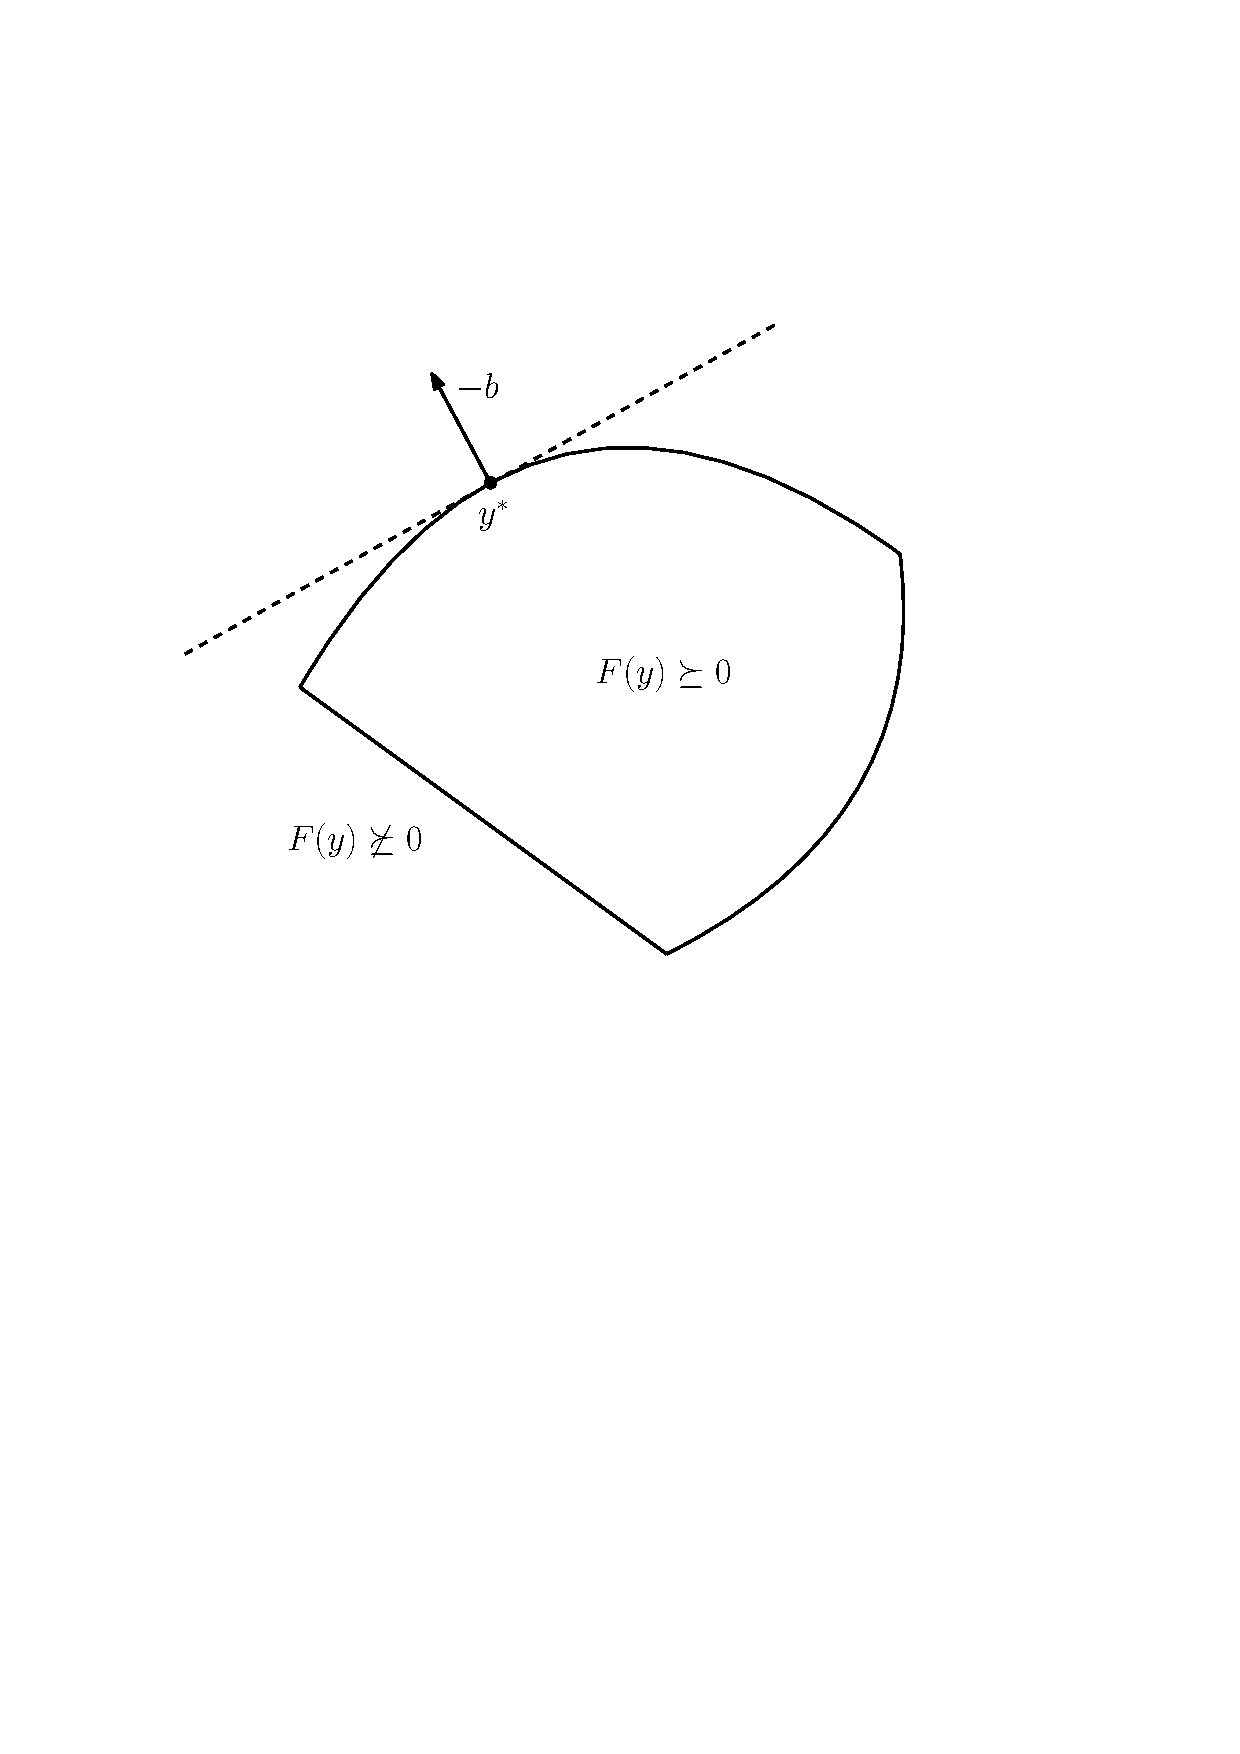
\includegraphics[width=0.5\textwidth]{drawings/SDP_problem.pdf}
  \caption{Example of a simple semidefinite problem for $y\in\R^2$. Boundary of the feasible set $\big\{y\ |\ F(y)\succeq 0\big\}$ is shown as a black curve. The minimal value of the objective function $b^\top y$ is attained at $y^*$.}
  \labelfig{SDP:prelim:problem}
\end{figure}

The optimal solution $y^*$ of any semidefinite program lies on the boundary of the feasible set, supposing the problem is feasible and the solution exists.
The boundary of the feasible set is not smooth in general, but it is piecewise smooth as each piece is an algebraic surface.

\begin{example}[Linear programming]
  Semidefinite programming can be seen as an extension to the linear programming since the componentwise inequalities between vectors in linear programming can be replaced by LMI.
  Consider a linear program in a standard form
  \begin{eqnarray}
    \begin{array}{rclrrclcll}
      y^* &=& \displaystyle \arg\min_{y\in\R^m} & \multicolumn{3}{l}{b^\top y} \\
      && \text{s.t.} & \displaystyle Ay - c &\geq& 0
    \end{array}
  \end{eqnarray}
  with $b\in\R^m$, $c\in\R^n$ and $A = \bmB a_1 & \ldots & a_m \bmE \in\R^{n\times m}$.
  This program can be transformed into the semidefinite program \refeqb{SDP:prelim:dual} by assigning
  \begin{eqnarray}
    C &=& \diag(c),\\
    A_i &=& \diag(a_i).
  \end{eqnarray}
\end{example}

\section{State of the art review}
An early paper by R. Bellman and K. Fan about theoretical properties of semidefinite programs \cite{Bellman-Fan} was issued in 1963.
Later on, many researchers worked on the problem of minimizing the maximal eigenvalue of a symmetric matrix, which can be done by solving a semidefinite program.
Selecting a few from many: J. Cullum, W. Donath, P. Wolfe \cite{Cullum-Donath-Wolfe}, M. Overton \cite{Overton} and G. Pataki \cite{Pataki}.
In 1984, the interior-point methods for LPs solving were introduced by N. Karmarkar \cite{Karmarkar1984}.
It was the first reasonably efficient algorithm that solves LPs in polynomial time with excellent behavior in practise.
The interior-point algorithms were then extended to be able to solve convex quadratic programs.

In 1988, Y. Nesterov and A. Nemirovski \cite{Nesterov-Nemirovski} did an important breakthrough.
They showed that interior-point methods developed for LPs solving can be generalized to all convex optimization problems.
All that is required, is the knowledge of a self-concordant barrier function for the feasible set of the problem.
Y. Nesterov and A. Nemirovski have shown that a self-concordant barrier function exists for every convex set.
However their proposed universal self-concordant barrier function and its first and second derivatives are not easily computable.
Fortunately, for SDP, which is an important class of convex optimization programs, computable self-concordant barrier functions are known, and therefore the interior-point methods can be used.

Nowadays, there are many libraries and toolboxes that one can use for solving semidefinite programs.
They differ to each other in used methods and their implementations.
Before starting solving a problem, one should know the details of the problem to solve and choose the library accordingly to it as not every method and its implementation is suitable for the given problem.

Most methods are based on interior-point methods, which are efficient and robust for general semidefinite programs.
The main disadvantage of these methods is that they need to store and factorize usually large Hessian matrix.
Most modern implementations of the interior-point methods do not need the knowledge of an interior feasible point in advance.
SeDuMi \cite{sedumi} casts the standard semidefinite program into the homogeneous self-dual form, which has a trivial feasible point.
SDPA \cite{sdpa} uses an infeasible interior-point method, which can initialized by an infeasible point.
Some of the libraries (e.g.\ MOSEK \cite{mosek}) have started out as LPs solvers and were extended for QCQPs solving and convex optimization later on.

Another type of methods used in SDP are the first-order methods. 
They avoid storing and factorizing Hessian matrices, and therefore they are able to solve much larger problems than interior-point methods, but at some cost in accuracy.
This method is implemented, for instance, in the SCS solver \cite{scs}.

\section{Nesterov's approach}
In this section, we will follow Chapter 4 of \cite{Nesterov-2004} by Y. Nesterov, which is devoted to the convex optimization problems.
This chapter describes the state of the art interior-point methods for solving convex optimization problems.
We will extract from it the only minimum, just to be able to introduce an algorithm for semidefinite programs solving.
We will present some basic definitions and theorems, but we will not prove them.
For the proofs and more details look into \cite{Nesterov-2004}.

\subsection{Self-concordant functions}
\begin{definition}[Self-concordant function in $\R$]
  A closed convex function $f: \R \mapsto \R$ is self-concordant if there exist a constant $M_f \geq 0$ such that the inequality
  \begin{eqnarray}
    |f'''(x)| &\leq& M_f f''(x)^{3/2}
  \end{eqnarray}
  holds for all $x\in\dom f$.
\end{definition}

For better understanding of self-concordant functions, we provide several examples.

\begin{example}~
  \begin{enumerate}
    \item Linear and convex quadratic functions.
      \begin{eqnarray}
        f'''(x) &=& 0\ \text{ for all } x
      \end{eqnarray}
      Linear and convex quadratic functions are self-concordant with constant $M_f = 0$.
    \item Negative logarithms.
      \begin{eqnarray}
        f(x) &=& -\ln(x)\ \text{ for } x>0\\
        f'(x) &=& -\frac{1}{x}\\
        f''(x) &=& \frac{1}{x^2}\\
        f'''(x) &=& -\frac{2}{x^3}\\
        \frac{|f'''(x)|}{f''(x)^{3/2}} &=& 2
      \end{eqnarray}
      Negative logarithms are self-concordant functions with constant $M_f = 2$.

    \item Exponential functions.
      \begin{eqnarray}
        f(x) &=& e^x\\
        f''(x) \ =\ f'''(x) &=& e^x\\
        \frac{|f'''(x)|}{f''(x)^{3/2}} &=& e^{-x/2} \rightarrow+\infty \ \text{ as } x\rightarrow-\infty
      \end{eqnarray}
      Exponential functions are not self-concordant functions.
  \end{enumerate}
\end{example}

\begin{definition}[Self-concordant function in $\R^n$]
  A closed convex function $f: \R^n \mapsto \R$ is self-concordant if function
  \begin{eqnarray}
    g(t) &=& f(x + tv)
  \end{eqnarray}
  is self-concordant for all $x\in\dom f$ and all $v\in\R^n$.
\end{definition}

Now, let us focus on the main properties of self-concordant functions.

\begin{theorem}
  Let functions $f_i$ be self-concordant with constants $M_i$  and let $\alpha_i > 0$, $i = 1,2$. Then the function
 \begin{eqnarray}
   f(x) &=& \alpha_1f_1(x) + \alpha_2f_2(x)
 \end{eqnarray}
 is self-concordant with constant
 \begin{eqnarray}
   M_f &=& \max \bigg\{\frac{1}{\sqrt{\alpha_1}}M_1, \frac{1}{\sqrt{\alpha_2}}M_2\bigg\}
 \end{eqnarray}
 and
 \begin{eqnarray}
   \dom f &=& \dom f_1 \cap \dom f_2.
 \end{eqnarray}
\end{theorem}

\begin{corollary}\labelcol{SDP:scf:scaling}
  Let function $f$ be self-concordant with some constant $M_f$ and $\alpha > 0$. Then the function $\phi(x) = \alpha f(x)$ is also self-concordant with the constant $M_\phi = \frac{1}{\sqrt{\alpha}}M_f$.
\end{corollary}

We call function $f(x)$ as the standard self-concordant function if $f(x)$ is some self-concordant function with the constant $M_f = 2$. Using \refcol{SDP:scf:scaling}, we can see that any self-concordant function can be transformed into the standard self-concordant function by scaling.

\begin{theorem}\labelthe{SDP:scf:hessian}
  Let function $f$ be self-concordant. If $\dom f$ contains no straight line, then the Hessian $f''(x)$ is nondegenerate at any $x$ from $\dom f$.
\end{theorem}

For some self-concordant function $f(x)$, for which we assume, that $\dom f$ contains no straight line (which implies that all $f''(x)$ are nondegenerate, see \refthe{SDP:scf:hessian}), we denote two local norms as
\begin{eqnarray}
  \| u \|_x &=& \sqrt{u^\top f''(x) u}\\
  \| u \|_x^* &=& \sqrt{u^\top f''(x)^{-1} u}.
\end{eqnarray}

Consider following minimization problem
\begin{eqnarray}
  x^* &=& \arg\min_{x\in\dom f} f(x)\labeleq{SDP:scf:minProblem}
\end{eqnarray}
as the minimization of the self-concordant function $f(x)$.
\refalg{SDP:scf} is describing the iterative process of solving optimization problem \refeqb{SDP:scf:minProblem}.
The algorithm is divided into two stages by the value of $\|f'(x_k)\|_{x_k}^*$.
The splitting parameter $\beta$ guarantees quadratic convergence rate for the second part of the algorithm. The parameter $\beta$ is chosen from interval $(0, \bar{\lambda})$, where
\begin{eqnarray}
  \bar{\lambda} &=& \frac{3 - \sqrt{5}}{2},
\end{eqnarray}
which is a root of the equation
\begin{eqnarray}
  \frac{\lambda}{(1-\lambda)^2} &=& 1.
\end{eqnarray}

\begin{algorithm}[ht]
  \begin{algorithmic}[1]
    \Require
      \Statex $f$ a self-concordant function to minimize
      \Statex $x_0 \in \dom f$ a starting point
      \Statex $\beta \in (0,\bar{\lambda})$ a parameter of size of the region of quadratic convergence
      \Statex $\varepsilon$ a precision
    \Ensure
      \Statex $x^*$ an optimal solution to the minimization problem \refeqb{SDP:scf:minProblem}
      \Statex

    \State $k \gets 0$
    \While{$\|f'(x_k)\|_{x_k}^* \geq \beta$} \labelalgline{SDP:scf:w1b}
      \State $x_{k+1} \gets x_k - \frac{1}{1+\|f'(x_k)\|_{x_k}^*}f''(x_k)^{-1}f'(x_k)$
      \State $k \gets k + 1$
    \EndWhile \labelalgline{SDP:scf:w1e}
    \While{$\|f'(x_k)\|_{x_k}^* > \varepsilon$} \labelalgline{SDP:scf:w2b}
      \State $x_{k+1} \gets x_k - f''(x_k)^{-1}f'(x_k)$
      \State $k \gets k + 1$
    \EndWhile \labelalgline{SDP:scf:w2e}
    \State \Return $x^* \gets x_k$

  \end{algorithmic}
  \caption{Newton method for minimization of the self-concordant functions.}
  \labelalg{SDP:scf}
\end{algorithm}


The first while loop (lines \refalgline{SDP:scf:w1b} -- \refalgline{SDP:scf:w1e}) represents damped Newton method, where at each iteration we have
\begin{eqnarray}
  f(x_k) - f(x_{k+1}) &\geq& \beta - \ln(1+\beta) \text{ for } k \geq 0,
\end{eqnarray}
where
\begin{eqnarray}
  \beta - \ln(1+\beta) &>& 0 \text{ for } \beta > 0,
\end{eqnarray}
and therefore the global convergence of the algorithm is ensured.
It can be shown that the local convergence rate of the damped Newton method is also quadratic, but the presented switching strategy is preferred as it gives better complexity bounds.

The second while loop of the algorithm (lines \refalgline{SDP:scf:w2b} -- \refalgline{SDP:scf:w2e}) is the standard Newton method with quadratic convergence rate.

The algorithm terminates when the required precision $\varepsilon$ is reached.


\subsection{Self-concordant barriers}
To be able to introduce self-concordant barriers, let us denote $\Dom f = \cl(\dom f)$.

\begin{definition}[Self-concordant barrier]\labeldef{SDP:scb:scb}
  Let $F(x)$ be a standard self-concordant function. We call it a $\nu$-self-concordant barrier for set $\Dom F$, if
  \begin{eqnarray}
    \sup_{u\in\R^n} \big(2u^\top F'(x) - u^\top F''(x) u\big) &\leq& \nu \labeleq{SDP:scb:def}
  \end{eqnarray}
  for all $x\in\dom F$. The value $\nu$ is called the parameter of the barrier.
\end{definition}

The inequality \refeqb{SDP:scb:def} can be rewritten into the following equivalent matrix notation:
\begin{eqnarray}
  F''(x) &\succeq& \frac{1}{\nu}F'(x)F'(x)^\top.\labeleq{SDP:scb:def1}
\end{eqnarray}

In \refdef{SDP:scb:scb}, the hessian $F''(x)$ is not required to be nondegenerate. However, in case that $F''(x)$ is nondegenerate, the inequality \refeqb{SDP:scb:def} is equivalent to
\begin{eqnarray}
  F'^\top(x)F''(x)^{-1}F'(x) &\leq& \nu.\labeleq{SDP:scb:def2}
\end{eqnarray}

Let us explore, which basic functions are self-concordant barriers.

\begin{example}~
  \begin{enumerate}
    \item Linear functions.
      \begin{eqnarray}
        F(x) &=& \alpha + a^\top x,\ \dom F = \R^n\\
        F''(x) &=& 0
      \end{eqnarray}
      From \refeqb{SDP:scb:def1} and for $a \neq 0$ follows, that linear functions are not self-concordant barriers.

    \item Convex quadratic functions.\\
      For $A = A^\top \succ 0$:
      \begin{eqnarray}
        F(x) &=& \alpha + a^\top x + \frac{1}{2} x^\top Ax,\ \dom F = \R^n\\
        F'(x) &=& a + Ax\\
        F''(x) &=& A
      \end{eqnarray}
      After substitution into \refeqb{SDP:scb:def2} we obtain
      \begin{eqnarray}
        (a + Ax)^\top A^{-1}(a + Ax) &=& a^\top A^{-1}a + 2a^\top x + x^\top Ax,
      \end{eqnarray}
      which is unbounded from above on $\R^n$. Therefore, quadratic functions are not self-concordant barriers.
      

    \item Logarithmic barrier for a ray.
      \begin{eqnarray}
        F(x) &=& -\ln x,\ \dom F = \big\{x\in\R\ |\ x > 0\big\}\\
        F'(x) &=& -\frac{1}{x}\\
        F''(x) &=& \frac{1}{x^2}
      \end{eqnarray}
      From \refeqb{SDP:scb:def2}, when $F'(x)$ and $F''(x)$ are both scalars, we get
      \begin{eqnarray}
        \frac{F'(x)^2}{F''(x)} &=& \frac{x^2}{x^2}\ =\ 1.
      \end{eqnarray}
      Therefore, the logarithmic barrier for a ray is a self-concordant barrier with parameter $\nu = 1$ on domain $\big\{x\in\R\ |\ x > 0\big\}$.
  \end{enumerate}
\end{example}

Now, let us focus on the main properties of self-concordant barriers.

\begin{theorem}\labelthe{SDP:scb:penaltyFunction}
  Let $F(x)$ be a self-concordant barrier. Then the function $c^\top x + F(x)$ is a self-concordant function on $\dom F$.
\end{theorem}

\begin{theorem}
  Let $F_i$ be $\nu_i$-self-concordant barriers, $i = 1,2$. Then the function
  \begin{eqnarray}
    F(x) &=& F_1(x) + F_2(x)
  \end{eqnarray}
  is a self-concordant barrier for convex set
  \begin{eqnarray}
    \Dom F &=& \Dom F_1 \cap \Dom F_2
  \end{eqnarray}
  with the parameter
  \begin{eqnarray}
    \nu &=& \nu_1 + \nu_2.
  \end{eqnarray}
\end{theorem}

\begin{theorem}\labelthe{SDP:scb:distance}
  Let $F(x)$ be a $\nu$-self-concordant barrier. Then for any $x\in\Dom F$ and $y\in\Dom F$ such that
  \begin{eqnarray}
    (y-x)^\top F'(x) &\geq& 0,
  \end{eqnarray}
  we have
  \begin{eqnarray}
    \|y-x\|_x &\leq& \nu + 2\sqrt{\nu}.
  \end{eqnarray}
\end{theorem}

There is one special point of convex set, which is important for solving convex minimization problem. 
It is called analytic center of convex set and we will focus on its properties.

\begin{definition}
  Let $F(x)$ be a $\nu$-self-concordant barrier for the set $\Dom F$. The point
  \begin{eqnarray}
    x^*_F &=& \arg \min_{x\in\Dom F} F(x) \labeleq{SDP:scb:ac}
  \end{eqnarray}
  is called the analytic center of convex set $\Dom F$, generated by the barrier $F(x)$.
\end{definition}

\begin{theorem}
  Assume that the analytic center of a $\nu$-self-concordant barrier $F(x)$ exists. Then for any $x\in\Dom F$ we have
  \begin{eqnarray}
    \|x-x^*_F\|_{x^*_F} &\leq& \nu + 2\sqrt{\nu}.
  \end{eqnarray}
\end{theorem}

This property clearly follows from \refthe{SDP:scb:distance} and the fact, that $F'(x^*_F) = 0$.

Thus, if $\Dom F$ contains no straight line, then the existence of $x^*_F$ (which leads to nondegenerate $F''(x^*_F)$) implies, that the set $\Dom F$ is bounded.

Now, we describe the algorithm and its properties for obtaining an approximation to the analytic center.
To find the analytic center, we need to solve the minimization problem \refeqb{SDP:scb:ac}.
For that, we will use the standard implementation of the damped Newton method with termination condition
\begin{eqnarray}
  \|F'(x_k)\|^*_{x_k} &\leq& \beta, \text{ for } \beta\in(0,1).
\end{eqnarray}
The pseudocode of the whole minimization process is shown in \refalg{SDP:scb:ac}.

\begin{algorithm}[ht]
  \begin{algorithmic}[1]
    \Require
      \Statex $F$ a self-concordant barrier
      \Statex $x_0 \in \Dom F$ a starting point
      \Statex $\beta \in (0,1)$ a centering parameter
    \Ensure
      \Statex $x^*_F$ an approximation of the analytic center of the set $\Dom F$
      \Statex

    \State $k \gets 0$
    \While{$\|F'(x_k)\|_{x_k}^* > \beta$}
      \State $x_{k+1} \gets x_k - \frac{1}{1+\|F'(x_k)\|_{x_k}^*}F''(x_k)^{-1}F'(x_k)$
      \State $k \gets k + 1$
    \EndWhile
    \State \Return $x^*_F \gets x_k$

  \end{algorithmic}
  \caption{Damped Newton method for analytic centers}
  \labelalg{SDP:scb:ac}
\end{algorithm}


\begin{theorem}
  \refalg{SDP:scb:ac} terminates no later than after $N$ steps, where
  \begin{eqnarray}
    N &=& \frac{1}{\beta - \ln(1+\beta)}\big(F(x_0) - F(x^*_F)\big).
  \end{eqnarray}
\end{theorem}

The knowledge of analytic center allows us to solve the standard minimization problem
\begin{eqnarray}
  x^* &=& \arg\min_{x\in Q} c^\top x \labeleq{SDP:scb:standardProblem}
\end{eqnarray}
with bounded closed convex set $Q \equiv \Dom F$, which has nonempty interior, and which is endowed with a $\nu$-self-concordant barrier $F(x)$.
Denote
\begin{eqnarray}
  f(t,x) &=& tc^\top x + F(x), \text{ for } t \geq 0
\end{eqnarray}
as a parametric penalty function.
Using \refthe{SDP:scb:penaltyFunction} we can see, that $f(t,x)$ is self-concordant in $x$.
Let us introduce new minimization problem using the parametric penalty function $f(t,x)$
\begin{eqnarray}
  x^*(t) &=& \arg\min_{x\in\dom F} f(t,x).\labeleq{SDP:scb:centralPath}
\end{eqnarray}
This trajectory is called the central path of the problem \refeqb{SDP:scb:standardProblem}.
We will reach the solution $x^*(t) \rightarrow x^*$ as $t \rightarrow +\infty$.
Moreover, since the set $Q$ is bounded, the analytic center $x^*_F$ of this set exists and
\begin{eqnarray}
  x^*(0) &=& x^*_F.
\end{eqnarray}
From the first-order optimality condition, any point of the central path satisfies equation
\begin{eqnarray}
  tc + F'\big(x^*(t)\big) &=& 0
\end{eqnarray}
Since the analytic center lies on the central path and can be found by \refalg{SDP:scb:ac}, all we have to do, to find the solution $x^*$, is to follow the central path. 
This enables us an approximate centering condition:
\begin{eqnarray}
  \|f'(t,x)\|^*_x\ =\ \|tc + F'(x)\|^*_x &\leq& \beta, \labeleq{SDP:scb:cntrCondition}
\end{eqnarray}
where the centering parameter $\beta$ is small enough.

Assuming $x\in\dom F$, one iteration of the path-following algorithm consists of two steps:
\begin{eqnarray}
  t_+ &=& t + \frac{\gamma}{\|c\|^*_x},\\
  x_+ &=& x - F''(x)^{-1}\big(t_+c+F'(x)\big).
\end{eqnarray}

\begin{theorem}
  Let $x$ satisfy the approximate centering condition \refeqb{SDP:scb:cntrCondition}
  \begin{eqnarray}
    \|tc + F'(x)\|^*_x &\leq& \beta
  \end{eqnarray}
  with $\beta < \bar{\lambda} = \frac{3-\sqrt{5}}{2}$.
  Then for $\gamma$, such that
  \begin{eqnarray}
    |\gamma| &\leq& \frac{\sqrt{\beta}}{1+\sqrt{\beta}} - \beta,
  \end{eqnarray}
  we have again
  \begin{eqnarray}
    \|t_+c + F'(x_+)\|^*_{x_+} &\leq& \beta.
  \end{eqnarray}
\end{theorem}

This theorem ensures the correctness of the presented iteration of the path-following algorithm.
For the whole description of the path-following algorithm please see \refalg{SDP:scb:pf}.

\begin{algorithm}[ht]
  \begin{algorithmic}[1]
    \Require
      \Statex $F$ a $\nu$-self-concordant barrier
      \Statex $x_0 \in \dom F$ a starting point satisfying $\|F'(x_0)\|^*_{x_0} \leq \beta$, e.g.\ the analytic center $x^*_F$ of the set $\Dom F$
      \Statex $\beta \in (0,1)$ a centering parameter
      \Statex $\gamma$ a parameter satisfying $|\gamma| \leq \frac{\sqrt{\beta}}{1+\sqrt{\beta}} - \beta$
      \Statex $\varepsilon > 0$ an accuracy
    \Ensure
      \Statex $x^*$ an approximation to the optimal solution to the minimization problem \refeqb{SDP:scb:standardProblem}
      \Statex

    \State $t_0 \gets 0$
    \State $k \gets 0$
    \While{$\varepsilon t_k < \nu + \frac{(\beta + \sqrt{\nu})\beta}{1-\beta}$}
      \State $t_{k+1} \gets t_k + \frac{\gamma}{\|c\|^*_{x_k}}$
      \State $x_{k+1} \gets x_k - F''(x_k)^{-1}\big(t_{k+1}c + F'(x_k)\big)$
      \State $k \gets k + 1$
    \EndWhile
    \State \Return $x^* \gets x_k$

  \end{algorithmic}
  \caption{Path following algorithm. \cite[Scheme~4.2.23]{Nesterov-2004}}
  \labelalg{SDP:scb:pf}
\end{algorithm}


\begin{theorem}
  \refalg{SDP:scb:pf} terminates no more than after $N$ steps, where
  \begin{eqnarray}
    N &\leq& \mathcal{O}\Bigg(\sqrt{\nu}\ln\frac{\nu \|c\|^*_{x^*_F}}{\epsilon}\Bigg).
  \end{eqnarray}
\end{theorem}

The parameters $\beta$ and $\gamma$ in \refalg{SDP:scb:ac} and \refalg{SDP:scb:pf} can be fixed. The reasonable values are:
\begin{eqnarray}
  \beta &=& \frac{1}{9},\labeleq{SDP:scb:beta}\\
  \gamma &=& \frac{\sqrt{\beta}}{1+\sqrt{\beta}} - \beta\ =\ \frac{5}{36}.\labeleq{SDP:scb:gamma}
\end{eqnarray}

The union of \refalg{SDP:scb:ac} and \refalg{SDP:scb:pf} can be easily used to solve the standard minimization problem \refeqb{SDP:scb:standardProblem}, supposing we have a feasible point $x_0\in Q$.

\subsection{Barrier function for semidefinite programming}
In this section, we are going to show, how to find a self-concordant barrier for the semidefinite program \refeqb{SDP:prelim:dual}, so that we can use \refalg{SDP:scb:ac} and \refalg{SDP:scb:pf} to solve it.
For the purpose of this section, we are interested only in the constrains of the problem.
The constrains are defining us the feasibility set $Q$:
\begin{eqnarray}
  Q &=& \bigg\{y\in\R^m\ |\ A_0 + \sum_{i=1}^mA_iy\ind i \succeq 0\bigg\},
\end{eqnarray}
where $A_0, \ldots, A_m \in\Sym^n$.
Let us denote $X(y) = A_0 + \sum_{i=1}^mA_iy\ind i$.
If the matrix $X(y)$ is block diagonal
\begin{eqnarray}
  X(y) &=& \begin{bmatrix}
          X_1(y) & 0      & \cdots & 0      \\
          0      & X_2(y) & \cdots & 0      \\
          \vdots & \vdots & \ddots & \vdots \\
          0      & 0      & \cdots & X_k(y)
        \end{bmatrix} \labeleq{SDP:bf:bd}
\end{eqnarray}
with $X_j(y)\in\Sym^{n_j}$ for $j = 1, \ldots, k$ and $\sum_{j=1}^k n_j = n$, then the feasibility set $Q$ can be expressed as
\begin{eqnarray}
  Q &=& \big\{y\in\R^m\ |\ X_j(y) \succeq 0,\ j = 1,\ldots, k\big\}.
\end{eqnarray}
This rule allows us to easily add or remove some constraints without touching the others and to keep the sizes of the used matrices small, which can significantly speed up the computation.

Instead of the set $Q$, which is parametrized by $y$, we can directly optimize over the set of positive semidefinite matrices. This set $\PSDCone^n$ is defined as
\begin{eqnarray}
  \PSDCone^n &=& \big\{X\in\Sym^n\ |\ X\succeq0\big\}
\end{eqnarray}
and it is called the cone of positive semidefinite $n\times n$ matrices. This cone is a closed convex set, which interior is formed by positive definite matrices and on its boundary lie matrices, which have at least one eigenvalue equal to zero.

Now, we are looking for a self-concordant barrier function, which will enable us to optimize over the cone $\PSDCone^n$.
The domain of this function needs to contain the set $\PSDCone^n$ and the values of the function have to be growing to $+\infty$ as we are getting closer to the boundary of the set $\PSDCone^n$.
This will create us a repelling force from the boundary of $\PSDCone^n$, when following the central path \refeqb{SDP:scb:centralPath}.
Consider the function $F(X)$ as the self-concordant barrier function for the set $\PSDCone^n$:
\begin{eqnarray}
  F(X) &=& -\ln\prod_{i=1}^{n}\lambda_i(X),
\end{eqnarray}
where $X\in\inter\PSDCone^n$ and $\big\{\lambda_i(X)\big\}_{i=1}^n$ is the set of eigenvalues of the matrix $X$.
To avoid the computation of eigenvalues, the function $F(X)$ can be also expressed as:
\begin{eqnarray}
  F(X) &=& -\ln\det(X).
\end{eqnarray}

\begin{theorem}\labelthe{SDP:bf:nu}
  Function $F(X)$ is an $n$-self-concordant barrier for $\PSDCone^n$.
\end{theorem}

\begin{example}
  Consider one-dimensional problem with linear constraint $x \geq 0$.
  Then, the set $Q$ is
  \begin{eqnarray}
    Q &=& \{x\in\R\ |\ x \geq 0\}
  \end{eqnarray}
  and one of the barrier functions for this set $Q$ is
  \begin{eqnarray}
    F(x) &=& -\ln(x).
  \end{eqnarray}
  Then, when following the central path \refeqb{SDP:scb:centralPath}, the function $F(x)$ allows us to reach the boundary of $Q$ as $t$ grows to $+\infty$.
  This situation is showed in \reffig{SDP:bf:barrier} for different values of $t$.

  \begin{figure}[ht]
    \centering
    \resizebox{0.95\textwidth}{!}{\input{graphs/SDP_barrier}}
    \caption{Illustration of the barrier function for different values of $t$.}
    \labelfig{SDP:bf:barrier}
  \end{figure}
\end{example}

Note, that $\Dom F \supseteq \PSDCone^n$ because $\det(X) \geq 0$ when the number of negative eigenvalues of $X$ is even. Therefore, the set $\Dom F$ is made by separated subsets, which one of them is $\PSDCone^n$. As \refalg{SDP:scb:ac} and \refalg{SDP:scb:pf} are interior point algorithms, when the starting point is from $\inter\PSDCone^n$, then we never leave $\PSDCone^n$ during the execution of the algorithms and the optimal solution is found.

Similarly, the self-concordant barrier function for the set $Q$ is a function 
\begin{eqnarray}
  F(y) &=& -\ln\det\big(X(y)\big). \labeleq{SDP:bf:bfy}
\end{eqnarray}

\begin{example}
  To make it clearer, what is the difference between the set $Q$ and $\Dom F(y)$, we have prepared this example. Let
  \begin{eqnarray}
    X(y) &=& \bmB y_2 & y_1 \\ y_1 & y_2 \bmE,
  \end{eqnarray}
  where $y = \bmB y_1 & y_2 \bmE^\top$. The equation
  \begin{eqnarray}
    z &=& \det(X(y))\ =\ y_2^2 - y_1^2
  \end{eqnarray}
  represents a hyperbolic paraboloid, which you can see in \reffig{SDP:bf:hyperPar}.
  Therefore, the equation $z = 0$ is a slice of it, denoted by the purple color in \reffig{SDP:bf:hyperParSlice}. The domain of the self-concordant barrier function is
  \begin{eqnarray}
    \Dom F(y) &=& \Big\{y\ |\ \det\big(X(y)\big) \geq 0\Big\}\labeleq{SDP:bf:domF}
  \end{eqnarray}
  and is shaded by the blue color.
  We can see, that the set $\Dom F(y)$ consists of two disjoint parts. One of them is the set, where $X(y)\succeq0$ (denoted by the orange color) and the second part is an area, where both eigenvalues of $X(y)$ are negative.
  Therefore, one has to pick his starting point $x_0$ from the interior of the set $Q$ to obtain the optimal solution from the set $Q$.

  \begin{figure}[ht]
    \centering
    \resizebox{0.95\textwidth}{!}{\input{graphs/SDP_hyperPar}}
    \caption{Hyperbolic paraboloid $z = y_2^2 - y_1^2$.}
    \labelfig{SDP:bf:hyperPar}
  \end{figure}

  \begin{figure}[ht]
    \centering
    \resizebox{0.95\textwidth}{!}{\input{graphs/SDP_hyperParSlice}}
    \caption{Illustration of the sets $\Dom F(y)$ and $\big\{y\ |\ X(y) \succeq 0\big\}$.}
    \labelfig{SDP:bf:hyperParSlice}
  \end{figure}
\end{example}

When the matrix $X$ has the block diagonal form \refeqb{SDP:bf:bd}, we can rewrite the barrier function \refeqb{SDP:bf:bfy} into summation form
\begin{eqnarray}
  F(y) &=& -\sum_{j=1}^k \ln\det\big(X_j(y)\big).
\end{eqnarray}
For the purposes of \refalg{SDP:scb:ac} and \refalg{SDP:scb:pf}, we need the first and the second partial derivatives of this function.
Let us denote $X_j(y) = A_{j, 0} + \sum_{i=1}^mA_{j, i}y\ind i$ for $j = 1, \ldots, k$, then the derivatives are:
\begin{eqnarray}
  \frac{\partial F}{\partial y\ind u}\big(y\big) &=& -\sum_{j=1}^k \tr\big(X_j(y)^{-1}A_{j,u}\big),\\
  \frac{\partial^2 F}{\partial y\ind u \partial y\ind v}\big(y\big) &=& \sum_{j=1}^k \tr\Big(\big(X_j(y)^{-1}A_{j,u}\big)\big(X_j(y)^{-1}A_{j,v}\big)\Big),
\end{eqnarray}
for $u, v = 1,\ldots, m$.

The computation of the derivatives is the most expensive part of each step of \refalg{SDP:scb:ac} and \refalg{SDP:scb:pf}.
Therefore, the estimated number of arithmetic operations of computation of the derivatives is also the complexity of each step in the algorithms.
The number of arithmetic operations for $j$-th constraint in form $\big\{y\ |\ X_j(y) \succeq 0\big\}$ is:
\begin{itemize}
  \item the computation of $X_j(y) = A_{j,0} + \sum_{i=1}^mA_{j,i}y\ind i$ needs $mn^2$ operations,
  \item the computation of the inversion $X_j(y)^{-1}$ needs $n^3$ operations,
  \item to compute all matrices $X_j(y)^{-1}A_{j,u}$ for $u = 1,\ldots,m$ is needed $mn^3$ operations,
  \item to compute $\tr\big(X_j(y)^{-1}A_{j,u}\big)$ for $u = 1,\ldots,m$ is needed $mn$ operations,
  \item the computation of $\tr\Big(\big(X_j(y)^{-1}A_{j,u}\big)\big(X_j(y)^{-1}A_{j,v}\big)\Big)$ for $u, v = 1,\ldots, m$ needs $m^2n^2$ operations.
\end{itemize}
The most expensive parts requires $mn^3$ and $m^2n^2$ arithmetic operations on each constraint.
Typically, the value $k$, the number of constraints, is small and it keeps constant, when the semidefinite programs are generated as subproblems, when solving more complex problems, e.g.\ polynomial optimization. Therefore, we can say, that $k$ is constant and we can omit it from the complexity estimation.
To sum up, one step of \refalg{SDP:scb:ac} and \refalg{SDP:scb:pf} requires
\begin{eqnarray}
  \mathcal{O}\big(m(m+n)n^2\big)
\end{eqnarray}
arithmetic operations.

\section{Implementation details}
To be able to study the algorithms described previously in this section, we have implemented them in the programming language Python \cite{python}.
The full knowledge of the code allows us to trace the algorithms step by step and inspect their behaviors.
Instead of using some state of the art toolboxes for semidefinite programming, e.g.\ SeDuMi \cite{sedumi} and MOSEK \cite{mosek}, which are more or less black boxes for us, the knowledge of the used algorithms allows us to decide, if the chosen algorithm is suitable for the given semidefinite problem or not.
Moreover, if we would like to create some specialized solver for some class of semidefinite problems, we can easily reuse the code, edit it as required and build the solver very quickly.
On the other hand, we can not expect that our implementation will be as fast as the implementation of some state of the art toolboxes, as much more time and people was used for developing them.

The implementation is compatible with Python version 3.6 and higher.
The package NumPy is used for linear algebra computations.
Please refer to the installation guide of NumPy for your system to ensure, that it is correctly set to use the linear algebra libraries, e.g.\ LAPACK \cite{lapack}, ATLAS \cite{atlas} and BLAS \cite{blas}.
The incorrect setting of these libraries causes significant drop of the performance.
Other Python packages are required as well, e.g.\ SymPy and SciPy, but theirs settings are not so crucial for the performance of this implementation.

\subsection{Package installation}
The package with implementation of \refalg{SDP:scb:ac} and \refalg{SDP:scb:pf} is named polyopt, as the semidefinite programming part of this package is only a tool, which is  used for polynomial optimization, which will be described in \refsec{poly}.
%TODO: ref to polymonial optimization section
The newest version of the package is available at \url{http://cmp.felk.cvut.cz/~trutmpav/master-thesis/polyopt/}.
To install the package on your system, you have to clone and checkout the Git repository with the source codes of the package.
To install other packages that are required, the preferred way is to use the pip\footnote{The PyPA recommended tool for installing Python packages. See \url{https://pip.pypa.io}.} installer. The required packages are listed in the \texttt{requirements.txt} file.
Then, install the package using the script \texttt{setup.py}.
For the exact commands for the whole installation process please see \reflis{SDP:imp:install}.
\begin{lstlisting}[language=bash, caption={Installation of the package polyopt.}, labellis={SDP:imp:install}]
git clone https://github.com/PavelTrutman/polyopt.git
cd polyopt
pip3 install -r requirements.txt
python3 setup.py install
\end{lstlisting}
To check, whether the installation was successful, run command \texttt{python3 setup.py test} and the predefined tests will be automatically run.
If no error emerges, then the package is installed and ready to use.

\subsection{Usage}
The polyopt package is created to be able to solve semidefinite programs in a form
\begin{eqnarray}
  \begin{array}{rclrrclcll}
    y^* &=& \displaystyle \arg\min_{y\in\R^m} & \multicolumn{3}{l}{c^\top y} \\
    && \text{s.t.} & \displaystyle A_{j,0} + \sum_{i=1}^m A_{j,i}y\ind i &\succeq& 0 \text{ for } j = 1,\ldots,k,
  \end{array}
\end{eqnarray}
where $A_{j,i}\in\Sym^{n_j}$ for $i = 0,\dots m$ and $j=1,\dots,k$, $c\in\R^m$ and $k$ is the number of constraints.
In addition, a strictly feasible point $y_0\in\R^m$ must be given.

The semidefinite program solver is implemented in the class \texttt{SDPSolver}. Firstly, the problem is initialized by the matrices $A_{j,i}$ and the vector $c$.
Then, the function \texttt{solve} is called with parameter $y_0$ as the starting point and with the method for the analytic center estimation.
A choice from two methods is available, firstly, the method \texttt{dampedNewton}, which corresponds to \refalg{SDP:scb:ac}, and secondly, the method \texttt{auxFollow}, which is the implementation of the Auxiliary path-following scheme \cite{Nesterov-2004}. 
However, the \texttt{auxFollow} method is unstable and it fails in some cases, and therefore it is not recommended to use.
The function \texttt{solve} returns the optimal solution $y^*$.
The minimal working example is shown in \reflis{SDP:imp:usage}.
\begin{lstlisting}[language=python, caption={Typical use of the class \texttt{SDPSolver} of the polyopt package.}, labellis={SDP:imp:usage}]
import polyopt

# supposing the matrices Aij and the vectors c and y0 are already defined
problem = polyopt.SDPSolver(c, [[A10, A11, ..., A1m], ..., [Ak0, Ak1, ..., Akm]])
yStar = problem.solve(y0, problem.dampedNewton)
\end{lstlisting}

Detailed info can be printed out during the execution of the algorithm.
This option can be set by \texttt{problem.setPrintOutput(True)}.
Then, in each iteration of \refalg{SDP:scb:ac} and \refalg{SDP:scb:pf}, the values $k$, $x_k$ and eigenvalues of $X_j(x_k)$ are printed.

If $n$, the dimension of the problem, is equal to 2, boundary of the set $\Dom F$ \refeqb{SDP:bf:domF} and all intermediate points $x_k$ can be plotted.
This can be enabled by setting \texttt{problem.setDrawPlot(True)}.
An example of such a graph is shown in \reffig{SDP:imp:demo}.

The parameters $\beta$ and $\gamma$ are predefined to the same values as in \refeqb{SDP:scb:beta} and \refeqb{SDP:scb:gamma}.
These parameters can be set to different values by assigning to the variables \texttt{problem.beta} and \texttt{problem.gamma} respectively.
The default value for the accuracy parameter $\epsilon$ is $10^{-3}$.
This value can be changed by overwriting the variable \texttt{problem.eps}.

The function \texttt{problem.getNu()} returns the $\nu$ parameter of the self-concordant barrier function used for the problem according to \refthe{SDP:bf:nu}.
When the problem is solved, we can obtain the eigenvalues of $X(y^*)$ by calling \texttt{problem.eigenvalues()}.
We should observe, that some of them are positive and some of them are zero (up to the numerical precision).
The zero eigenvalues mean, that we have reached the boundary of the set $Q$, because the optimal solution lies always on the boundary of the set $Q$.

It may happen, that the set $\Dom F$ is not bounded, but the optimal solution can be attained.
In this case, the analytic center does not exists and the proposed algorithms can not be used. 
By adding a constraint 
\begin{eqnarray}
  X_{k+1}(y) &=& \bmB R^2 & y\ind1 & y\ind2 & \cdots & y\ind m\\
                      y\ind1 & 1 & 0 & \cdots & 0\\
                      y\ind2 & 0 & 1 & \cdots & 0\\
                      \vdots & \vdots & \vdots & \ddots & \vdots\\
                      y\ind m & 0 & 0 & \cdots & 1\bmE \text{ for } R\in\R, \labeleq{SDP:imp:bound}
\end{eqnarray}
we bound the set by the ball with radius $R$.
The constraint \refeqb{SDP:imp:bound} is equivalent to
\begin{eqnarray}
  \|y\|_2^2 &\leq&R^2.
\end{eqnarray}
This will make the set $\Dom F$ bounded and the analytic center can by found in the standard way by \refalg{SDP:scb:ac}.
When optimizing the linear function by \refalg{SDP:scb:pf}, the radius $R$ may be set too small and the optimum may be found on the boundary of the constraint \refeqb{SDP:imp:bound}.
Then, the found optimum is not the solution of the original problem and the algorithm has to be run again with bigger value of $R$.
The optimum is found on the boundary of the constraint \refeqb{SDP:imp:bound}, if at least one of the eigenvalues of $X_{k+1}(y^*)$ is zero.
In our implementation, the artificial bounding constraint \refeqb{SDP:imp:bound} can be set by \texttt{problem.bound(R)}.
When the problem is solved, we can list the eigenvalues of $X_{k+1}(y^*)$ by the function \texttt{problem.eigenvalues('bounded')}.

\begin{example}\labelex{SDP:imp:demo}
  Let us present a simple example to show a detailed usage of the package polyopt.
  Let us have semidefinite program in a form
  \begin{eqnarray}
    \begin{array}{rclrrclcll}
      y^* &=& \displaystyle \arg\min_{y\in\R^2} & \multicolumn{3}{l}{y\ind1 + y\ind2} \\
      && \text{s.t.} & \displaystyle \bmB 1 +y\ind1 & y\ind2 & 0\\ y\ind2 & 1 -y\ind1& y\ind2\\ 0 & y\ind2 & 1-y\ind1 \bmE &\succeq& 0
    \end{array}
    \end{eqnarray}
  with starting point
  \begin{eqnarray}
    y_0 &=& \bmB 0 & 0\bmE^\top.
  \end{eqnarray}
  \reflis{SDP:imp:demo} shows the Python code used to solve the given problem.
  The graph of the problem is showed in \reffig{SDP:imp:demo}.
  The analytic center of the feasible region of the problem is
  \begin{eqnarray}
    y_F^* &=& \bmB -0.317 & 0\bmE^\top,
  \end{eqnarray}
  the optimal solution is attained at
  \begin{eqnarray}
    y^* &=& \bmB -0.778 & -0.592 \bmE^\top
  \end{eqnarray}
  and the objective function has value $-1.37$.
  The eigenvalues of $X(y^*)$ are
  \begin{eqnarray}
    \Big\{\lambda_i\big(X(y^*)\big)\Big\}_{i=1}^3 &=& \{2.32\cdot10^{-4};\ 1.32;\ 2.45\}.
  \end{eqnarray}

  \begin{lstlisting}[float, language=python, caption={Code for solving semidefinite problem stated in \refex{SDP:imp:demo}.}, labellis={SDP:imp:demo}]
from numpy import *
import polyopt

# Problem statement
# min c1*y1 + c2*y2
# s.t. A0 + A1*y1 + A2*y2 >= 0
c = array([[1], [1]])
A0 = array([[1,  0,  0],
            [0,  1,  0],
            [0,  0,  1]])
A1 = array([[1,  0,  0],
            [0, -1,  0],
            [0,  0, -1]])
A2 = array([[0,  1,  0],
            [1,  0,  1],
            [0,  1,  0]])

# starting point 
y0 = array([[0], [0]])

# create the solver object
problem = polyopt.SDPSolver(c, [[A0, A1, A2]])

# enable graphs
problem.setDrawPlot(True)

# enable informative output
problem.setPrintOutput(True)

# solve!
yStar = problem.solve(y0, problem.dampedNewton)

# print eigenvalues of X(yStar)
print(problem.eigenvalues())
  \end{lstlisting}

  \begin{figure}[ht]
    \centering
    \resizebox{0.95\textwidth}{!}{\input{graphs/SDP_demo}}
    \caption{Graph of the semidefinite optimization problem stated in \refex{SDP:imp:demo}.}
    \labelfig{SDP:imp:demo}
  \end{figure}
\end{example}

\section{Comparison with the state of the art methods}
%TODO some graphs



\chapter{Optimization over polynomials}\labelcha{POP}
This chapter is devoted to the application of semidefinite programming in polynomial algebra.
Firstly, we introduce basic notation from the polynomial algebra and the state of the art method for solving systems of polynomial equations using so called multiplication matrices.
Then we introduce the theory of moment matrices, since moment matrices will be used to relax the polynomial problems into the semidefinite ones.
After that, we will focus on polynomial optimization, i.e.\ optimizing a polynomial function given polynomial constrains.
We will present a method, how to use hierarchies of semidefinite problems to solve a polynomial optimization problem.
We implement this method and compare it to the state of the art optimization toolboxes.
In the last section of this chapter, we will introduce the moment method for polynomial systems solving.
This method also uses hierarchies of semidefinite problems to solve the polynomial systems with the advantage that only real solutions are found.
Since when solving polynomial systems arisen from computer vision geometry, we are typically interested only in the real solutions, this method may prove to be a useful tool to eliminate the non-real solutions.

\section{Algebraic preliminaries}
In this whole chapter focused on polynomial optimization and polynomial systems solving, we will follow the notation from \cite{Cox-Little-Shea97}.
Just to keep this chapter self-contained, we will recall some basics of polynomial algebra.

\subsection{The polynomial ring, ideals and varieties}
Firstly, the ring of multivariate polynomials in $n$ variables with coefficients in $\R$ is denoted as $\R[x]$, where $x = \bmB x_1 & x_2 & \cdots & x_n \bmE^\top$.
For $\alpha_1, \alpha_2, \ldots, \alpha_n\in\N$, $x^\alpha$ denotes the monomial ${x_1}^{\alpha_1}\cdot{x_2}^{\alpha_2}\cdot\cdots\cdot{x_n}^{\alpha_n}$, with a total degree $|\alpha| = \sum_{i=1}^n \alpha_i$, where $\alpha = \bmB \alpha_1 & \alpha_2 & \cdots & \alpha_n\bmE^\top$.
A polynomial $p\in\R[x]$ can be written as
\begin{align}
  p &= \sum_{\alpha\in\N^n} p_\alpha x^\alpha \labeleq{POP:pal:pol}
\end{align}
with a total degree $\deg(p) = \max_{\alpha\in\N^n}|\alpha|$ for non-zero coefficients $p_\alpha\in\R$.

A linear subspace $I \subseteq \R[x]$ is an ideal if $p\in I$ and $q\in\R[x]$ implies $pq \in I$.
Let $f_1, f_2, \ldots, f_m$ be polynomials in $\R[x]$. Then the set
\begin{align}
  \langle f_1, f_2, \ldots, f_m\rangle &= \Bigg\{\sum_{j=1}^mh_jf_j\ |\ h_1, h_2, \ldots, h_m\in\R[x]\Bigg\}
\end{align}
is called the ideal generated by $f_1, f_2, \ldots, f_m$.
Given the ideal $I\in\R[x]$, the algebraic variety of $I$ is the set
\begin{align}
  V_\C(I) &= \big\{x\in\C^n\ |\ f(x) = 0 \text{ for all } f\in I\big\}
\end{align}
and its real variety is
\begin{align}
  V_\R(I) &= V_\C(I) \cap \R^n.
\end{align}
The ideal $I$ is said to be zero-dimensional when its complex variety $V_\C(I)$ is finite.
The vanishing ideal of a subset $V\subseteq\C^n$ is the ideal
\begin{align}
  \Ideal(V) &= \big\{f\in\R[x]\ |\ f(x) = 0 \text{ for all } x\in V\big\}.
\end{align}
The radical ideal of the ideal $I\subseteq \R[x]$ is the ideal
\begin{align}
  \sqrt{I} &= \big\{f\in\R[x]\ |\ f^m\in I \text{ for some } m\in\Z^+\big\}.
\end{align}
The real radical ideal of the ideal $I\subseteq \R[x]$ is the ideal
\begin{align}
  \sqrt[\R]{I} &= \big\{f\in\R[x]\ |\ f^{2m} + \sum_j h_j^2 \in I \text{ for some } h_j\in\R[x], m\in\Z^+\big\}.
\end{align}

The following two theorems are stating the relations between the vanishing and (real) radical ideals.

\begin{theorem}[Hilbert's Nullstellensatz]
  Let $I\in\R[x]$ be an ideal. The radical ideal of $I$ is equal to the vanishing ideal of its variety, i.e.\
  \begin{align}
    \sqrt{I} &= \Ideal\big(V_\C(I)\big).
  \end{align}
\end{theorem}

\begin{theorem}[Real Nullstellensatz]
  Let $I\in\R[x]$ be an ideal. The real radical ideal of $I$ is equal to the vanishing ideal of its real variety, i.e.\
  \begin{align}
    \sqrt[\R]{I} &= \Ideal\big(V_\R(I)\big).
  \end{align}
\end{theorem}

The quotient ring $\R[x]/I$ is the set of all equivalence classes of polynomials in $\R[x]$ for congruence modulo ideal $I$
\begin{align}
  \R[x]/I &= \big\{\![f]\ |\ f\in\R[x]\!\big\},
\end{align}
where the equivalence class $[f]$ is
\begin{align}
  [f] &= \big\{f+g\ |\ g\in I\big\}.
\end{align}
Because $\R[x]/I$ is a ring, it is equipped with addition and multiplication on the equivalence classes:
\begin{align}
  [f] + [g] &= [f + g],\\
  ~[f][g] &= [fg]
\end{align}
for $f, g\in\R[x]$.

For zero-dimensional ideal $I$, there is a relation between the dimension of $\R[x]/I$ and the cardinality of the variety $V_\C(I)$:
\begin{align}
  |V_\C(I)| &\leq \dim\!\big(\R[x]/I\big).
\end{align}
Moreover, if $I$ is a radical ideal, then
\begin{align}
  |V_\C(I)| &= \dim\!\big(\R[x]/I\big).
\end{align}

Assume that the number of complex roots is finite and let $N = \dim\!\big(\R[x]/I\big)$, and therefore $|V_\C(I)|\leq N$.
Consider a set $\Base = \{b_1, b_2, \ldots, b_N\} \subseteq \R[x]$ for which the equivalence classes $[b_1], [b_2], \ldots, [b_N]$ are pairwise distinct and $\big\{\![b_1], [b_2], \ldots, [b_N]\!\big\}$ is a basis of $\R[x]/I$.
Then every polynomial $f\in\R[x]$ can be written in a unique way as
\begin{align}
  f &= \sum_{i=1}^Nc_ib_i + p,
\end{align}
where $c_i\in\R$ and $p\in I$.
The normal form of the polynomial $f$ modulo $I$ with respect to the basis $\Base$ is the polynomial
\begin{align}
  \NF_\Base(f) &= \sum_{i=1}^N c_ib_i.
\end{align}

\subsection{Solving systems of polynomial equations using multiplication matrices}
Systems of polynomial equations can be solved by computing eigenvalues and eigenvectors of so called multiplication matrices.
Given $f\in\R[x]$, we define the multiplication operator (by $f$) $\MM_f: \R[x]/I \rightarrow \R[x]/I$ as
\begin{align}
  \MM_f([g]) &= [f][g] = [fg].
\end{align}
It can be shown that $\MM_f$ is a linear mapping, and therefore can be represented by its matrix with respect to the basis $\Base$ of $\R[x]/I$.
For simplicity, we again denote this matrix $\MM_f$ and it is called the multiplication matrix by $f$.
When $\Base = \{b_1, b_2, \ldots, b_N\}$ and we set $\NF_\Base(fb_j) = \sum_{i=1}^N a_{i,j}b_i$ for $a_{ij}\in\R$, then the multiplication matrix is
\begin{align}
  \MM_f &= \bmB a_{1,1} & a_{1,2} & \cdots & a_{1,N}\\
                a_{2,1} & a_{2,2} & \cdots & a_{2,N}\\
                \vdots & \vdots & \ddots & \vdots\\
                a_{N,1} & a_{N,2} & \cdots & a_{N,N}\bmE.
\end{align}

\begin{theorem}[Stickelberger theorem]
  Let $I$ be a zero-dimensional ideal in $\R[x]$, let $\Base = \{b_1, b_2, \dots, b_N\}$ be a basis of $\R[x]/I$, and let $f\in\R[x]$.
  The eigenvalues of the multiplication matrix $\MM_f$ are the evaluations $f(v)$ of the polynomial $f$ at the points $v\in V_\C(I)$.
  Moreover, for all $v\in V_\C(I)$,
  \begin{align}
    (\MM_f)^\top[v]_\Base &= f(v)[v]_\Base,
  \end{align}
  setting $[v]_\Base = \bmB b_1(v) & b_2(v) & \cdots & b_N(v)\bmE^\top$; that is, the vector $[v]_\Base$ is a left eigenvector with eigenvalue $f(v)$ of the multiplication matrix $\MM_f$.
\end{theorem}

Therefore, we can create the multiplication matrix $\MM_{x_i}$ for the variable $x_i$ and then the eigenvalues of $\MM_{x_i}$ correspond to the $x_i$-coordinates of the points $V_\C(I)$.
This means that the solutions of the whole system can be found by computing eigenvalues $\lambda_{x_i} = \big\{\lambda_j(\MM_{x_i})\big\}_{j=1}^N$ of the multiplication matrix $\MM_{x_i}$ for all variables $x_i$.
Then $V_\C(I)$ is a subset of the Cartesian product $\lambda_{x_1} \times \lambda_{x_2} \times \cdots \times \lambda_{x_n}$ and one has to select only the points that are solutions.
However, this method becomes inefficient for large $n$, the number of variables, since $n$ multiplication matrices have to be constructed and their eigenvalues computed.

For this reason, the second property of multiplication matrices is used.
The roots can be recovered from the left eigenvectors of $\MM_f$, when all left eigenspaces of $\MM_f$ have dimension one.
This is the case, when the values $f(v)$ for $v\in V_\C(I)$ are pairwise distinct and when the ideal $I$ is radical.
In that case, each left eigenvector of $\MM_f$ corresponds to one solution $v\in V_\C(I)$ and the values of the eigenvectors are the evaluations $b_i(v)$ for $b_i\in\Base$, and therefore when the variable $x_i\in\Base$, we can readily obtain its value.

\begin{example}\labelex{POP:mm:ellhyp}
  Let us have a system of two polynomial equations.
  \begin{alignat}{7}
    {}-{}20 & x^2 & {}+{}   & xy & {}-{}12 & y^2 & {}-{}16 & x & {}-{}   & y & {}+{}48 & {}={} & 0 \labeleq{POP:mm:example1}\\
    12      & x^2 & {}-{}58 & xy & {}+{}3  & y^2 & {}+{}46 & x & {}-{}47 & y & {}+{}44 & {}={} & 0 \labeleq{POP:mm:example2}
  \end{alignat}
  The first equation represents an ellipse and the second one a hyperbola as you can see in \reffig{POP:mm:example}.
  Let us solve the system using multiplication matrices.

  \begin{figure}[ht]
    \centering
    \resizebox{0.95\textwidth}{!}{\input{graphs/POP_multiplicationMatrices}}
    \caption{The intersection of the ellipse \refeqb{POP:mm:example1} and the hyperbola \refeqb{POP:mm:example2} with solutions found by the eigenvalue and the eigenvector methods using multiplication matrices.}
    \labelfig{POP:mm:example}
  \end{figure}

  First of all, we have to compute the Gr\"obner basis \cite{Becker93} of the ideal, for example using the $F_4$ Algorithm \cite{F4}.
  We have got the following basis:
  \begin{alignat}{5}
    164 & x^2 & {}+{}99 & y^2 & {}+{}126 & x & {}+{}15  & y & {}-{}404,\\
    41  & xy  & {}+{}3  & y^2 & {}-{}16  & x & {}+{}34  & y & {}-{}52, \\
    41  & y^3 & {}-{}15 & y^2 & {}+{}48  & x & {}-{}170 & y & {}+{}96.
  \end{alignat}
  Now, we can select the monomial basis $\Base$
  \begin{align}
    \Base = \bmB 1 & y & x & y^2 \bmE^\top
  \end{align}
  and construct the multiplication matrices $\MM_x$ and $\MM_y$ accordingly, knowing that
  \begin{alignat}{6}
    \MM_x\Big(\!\big[1\big]\!\Big)   & {}={} & \big[x\big]    & {}={} &                     &               & 1                  & \big[x\big], &                     &             &                     &            \\
    \MM_x\Big(\!\big[y\big]\!\Big)   & {}={} & \big[xy\big]   & {}={} & {}-{}\frac{3}{41}   & \big[y^2\big] & {}+{}\frac{26}{41} & \big[x\big]  & {}-{}\frac{34}{41}  & \big[y\big] & {}+{}\frac{52}{41}  & \big[1\big],\\
    \MM_x\Big(\!\big[x\big]\!\Big)   & {}={} & \big[x^2\big]  & {}={} & {}-{}\frac{99}{164} & \big[y^2\big] & {}-{}\frac{63}{82} & \big[x\big]  & {}-{}\frac{15}{164} & \big[y\big] & {}+{}\frac{101}{41} & \big[1\big],\\
    \MM_x\Big(\!\big[y^2\big]\!\Big) & {}={} & \big[xy^2\big] & {}={} & {}-{}\frac{37}{41}  & \big[y^2\big] & {}+{}\frac{20}{41} & \big[x\big]  & {}+{}\frac{18}{41}  & \big[y\big] & {}+{}\frac{40}{41}  & \big[1\big],
  \end{alignat}
  and
  \begin{alignat}{6}
    \MM_y\Big(\!\big[1\big]\!\Big)   & {}={} & \big[y\big]   & {}={} &                   &                &                    &             &                   1 & \big[y\big], &                    &            \\
    \MM_y\Big(\!\big[y\big]\!\Big)   & {}={} & \big[y^2\big] & {}={} &                 1 & \big[y^2\big], &                    &             &                     &              &                    &            \\
    \MM_y\Big(\!\big[x\big]\!\Big)   & {}={} & \big[xy\big]  & {}={} & {}-{}\frac{3}{41} & \big[y^2\big]  & {}+{}\frac{26}{41} & \big[x\big] & {}-{}\frac{34}{41}  & \big[y\big]  & {}+{}\frac{52}{41} & \big[1\big],\\
    \MM_y\Big(\!\big[y^2\big]\!\Big) & {}={} & \big[y^3\big] & {}={} & \frac{15}{41}     & \big[y^2\big]  & {}-{}\frac{48}{41} & \big[x\big] & {}+{}\frac{170}{41} & \big[y\big]  & {}-{}\frac{96}{41} & \big[1\big].
  \end{alignat}
  Then, the multiplication matrices are:
  \begin{align}
    \MM_x &= \bmB 0 & \frac{52}{41} & \frac{101}{41} & \frac{40}{41}\\
                  0 & -\frac{34}{41} & -\frac{15}{164} & \frac{18}{41}\\
                  1 & \frac{26}{41} & -\frac{63}{82} & \frac{20}{41}\\
                  0 & -\frac{3}{41} & -\frac{99}{164} & -\frac{37}{41}\bmE,\\
    \MM_y &= \bmB 0 & 0 & \frac{52}{41} & -\frac{96}{41}\\
                  1 & 0 & -\frac{34}{41} & \frac{170}{41}\\
                  0 & 0 & \frac{26}{41} & -\frac{48}{41}\\
                  0 & 1 & -\frac{3}{41} & \frac{15}{41}\bmE.
  \end{align}
  The eigenvalues of $\MM_x$ and $\MM_y$ are
  \begin{align}
    \big\{\lambda_i(\MM_x)\big\}_{i=1}^4 &= \left\{-2;\ -1;\ -\frac{1}{2};\ 1\right\},\\
    \big\{\lambda_i(\MM_y)\big\}_{i=1}^4 &= \{-2;\ 0;\ 1;\ 2\}.
  \end{align}
  Therefore, there are $4\times4=16$ possible solutions of the system and we must verify, which of them are true solutions.
  Let us denote the set of all possible solutions as $\tilde{V}_\C(I)$.
  These possible solutions are shown in \reffig{POP:mm:example} by the blue color.

  Secondly, we compute the left eigenvectors of the multiplication matrix $\MM_x$ such that their first coordinates are ones, as it corresponds to the constant polynomial $b_1 = 1$.
  We obtain following four eigenvectors corresponding to four different solutions:
  \begin{align}
    \bmB 1\\ 1\\ 1\\ 1 \bmE,\
    \bmB 1\\ 0\\ -2\\ 0 \bmE,\
    \bmB 1\\ 2\\ -\frac{1}{2}\\ 4 \bmE,\
    \bmB 1\\ -2\\ -1\\ 4 \bmE.
  \end{align}
  Since the second and the third coordinate corresponds to $b_2 = y$ and $b_3 = x$ respectively, we have got four solutions to the system of polynomials \refeqb{POP:mm:example1} and \refeqb{POP:mm:example2}:
  \begin{align}
    V_\C(I) &= \left\{\!
        \bmB 1\\ 1 \bmE;\
        \bmB -2\\ 0 \bmE;\
        \bmB -\frac{1}{2}\\ 2 \bmE;\
        \bmB -1\\ -2 \bmE
      \!\right\}.
  \end{align}
  These solutions are shown by the orange color in \reffig{POP:mm:example}.
\end{example}

\section{Moment matrices}\labelsec{POP:MM}
Polynomial optimization and solving systems of polynomial equations via hierarchies of semidefinite programs is based on the theory of measures and moments.
But to keep the scope simple, we will avoid to introduce this theory.
However, since it provides better understanding of the matter, interested reader may look into \cite{SOS}.
Moreover, we will introduce the only minimal basics to be able to proceed with polynomial optimization and polynomial systems solving.
More and detailed information can be found in \cite{SOS} too.

Now, let us start with the theory about moment matrices, which are crucial for the application of SDP on polynomial optimization and polynomial systems solving.
Recall that a polynomial has a form \refeqb{POP:pal:pol}.
Since such a polynomial may have infinite number of coefficients, let us introduce a polynomial $p\in\R[x]$ of the degree $d\in\N$:
\begin{align}
  p(x) &= \sum_{\alpha\in\N_d^n}p_\alpha x^\alpha,
\end{align}
where $\N_d$ are natural numbers (including zero) up to the number $d$.
This polynomial has at most $\binom{n+d}{n}$ non-zero coefficients, since there are $\binom{n+d}{n}$ monomials in $n$ variables up to degree $d$.
We will use the notation $\vc(p)$ for the vector of the coefficients of the polynomial $p$ with respect to some monomial basis $\Base$:
\begin{align}
  \vc(p)\ind{\alpha} &= p_\alpha
\end{align}
for $\alpha\in\N_d^n$.

\begin{definition}[Riesz functional]
  Given a sequence $y\ind\alpha = y_\alpha$ for $\alpha\in\N^n$, we define the Riesz linear functional $\ell_y: \R[x]\rightarrow\R$ such that
  \begin{align}
    \ell_y(x^\alpha) &= y_\alpha
  \end{align}
  for all $\alpha\in\N^n$.
\end{definition}
The linearity of the Riesz functional allows us to apply it on polynomials.
\begin{align}
  \ell_y\big(p(x)\big) = \ell_y\!\left(\sum_{\alpha\in\N_d^n}p_\alpha x^\alpha\!\right) = \sum_{\alpha\in\N_d^n}p_\alpha \ell_y(x^\alpha) = \sum_{\alpha\in\N_d^n}p_\alpha y_\alpha
\end{align}
From the equation above, we can see that Riesz functional substitutes a new variable $y_\alpha$ for each monomial $x^\alpha$, and therefore we can interpret the Riesz functional as an operator that linearizes polynomials. 

\begin{example}
  Given polynomial $p\in\R[x_1, x_2]$
  \begin{align}
    p(x) &= x_1^2 + 3x_1x_2 - 7x_2 + 9
  \end{align}
  with $\deg(p) = 2$, the vector of its coefficients with respect to monomial basis
  \begin{align}
    \Base &= \bmB x_1^2 & x_1x_2 & x_2^2 & x_1 & x_2 & 1\bmE^\top
  \end{align}
  is
  \begin{align}
    \vc(p) &= \bmB 1 & 3 & 0 & 0 & -7 & 9\bmE^\top.
  \end{align}
  The Riesz functional of $p(x)$ is
  \begin{align}
    \ell\big(p(x)\big) &= y_{20} + 3y_{11} -7y_{01} + 9y_{00}.
  \end{align}
\end{example}

\begin{definition}[Moment matrix]\labeldef{POP:MM}
  A symmetric matrix $M$ indexed by $\N^n$ is said to be a moment matrix (or generalized Hankel matrix) if its $(\alpha, \beta)$-entry depends only on the sum $\alpha + \beta$ of the indices.
  Given sequence $y\ind\alpha = y_\alpha$ for $\alpha\in\N^n$, the moment matrix $M(y)$ has form
  \begin{align}
    M(y)\ind{\alpha, \beta} &= y_{\alpha + \beta}
  \end{align}
  for $\alpha, \beta \in\N^n$.
\end{definition}

\begin{definition}[Truncated moment matrix]
  Given sequence $y\ind\alpha = y_\alpha$ for $\alpha\in\N^n$, the truncated moment matrix $M_s(y)$ of order $s\in\N$ has form
  \begin{align}
    M_s(y)\ind{\alpha, \beta} &= y_{\alpha + \beta}
  \end{align}
  for $\alpha, \beta \in\N_s^n$.
\end{definition}

The moment matrices are linear in $y$ and symmetric, we can see that
\begin{align}
  M_s(y)\in\Sym^{\binom{n+s}{n}}
\end{align}
since $\binom{n+s}{n}$ is the number of monomials in $n$ variables up to degree $s$.

\begin{example}
  For $n=2$, the moment matrices for different orders are:
  \begin{align}
    M_0(y) &= \bmB y_{00} \bmE,\\
    M_1(y) &= \bmdB{c:cc}
                y_{00} & y_{10} & y_{01}\\\hdashline
                y_{10} & y_{20} & y_{11}\\
                y_{01} & y_{11} & y_{02}
              \bmdE,\\
    M_2(y) &= \bmdB{c:cc:ccc}
                y_{00} & y_{10} & y_{01} & y_{20} & y_{11} & y_{02}\\\hdashline
                y_{10} & y_{20} & y_{11} & y_{30} & y_{21} & y_{12}\\
                y_{01} & y_{11} & y_{02} & y_{21} & y_{12} & y_{03}\\\hdashline
                y_{20} & y_{30} & y_{21} & y_{40} & y_{31} & y_{22}\\
                y_{11} & y_{21} & y_{12} & y_{31} & y_{22} & y_{13}\\
                y_{02} & y_{12} & y_{03} & y_{22} & y_{13} & y_{04}
              \bmdE.
  \end{align}
  All the elements in the blocks separated by the dashed lines have the same degree.
  Moreover, we can see that the moment matrices of smaller order are nothing more than submatrices of the moment matrices of bigger order.

  And just one example for $n=3$:
  \begin{align}
    M_1(y) &= \bmdB{c:ccc}
                y_{000} & y_{100} & y_{010} & y_{001}\\\hdashline
                y_{100} & y_{200} & y_{110} & y_{101}\\
                y_{010} & y_{110} & y_{020} & y_{011}\\
                y_{001} & y_{101} & y_{011} & y_{002}
              \bmdE.
  \end{align}
\end{example}

\begin{definition}[Localizing matrix]
  Given sequence $y\ind\alpha = y_\alpha$ for $\alpha\in\N^n$ and polynomial $q(x)\in\R[x]$, its localizing matrix $M_s(qy)$ of order $s$ has form
  \begin{align}
    M_s(qy)\ind{\alpha,\beta} &= \sum_\gamma q_\gamma y_{\alpha + \beta + \gamma}
  \end{align}
  for $\alpha, \beta \in\N_s^n$.
\end{definition}

Notation $M_s(qy)$ emphasis that the localizing matrix is bilinear in $q$ and $y$.

\begin{example}
  For $n = 2$ and a polynomial $q(x) = x_1x_2 + 2x_1 + 3$, the localizing matrix of order one is
  \begin{align}
    M_1(qy) &= \bmdB{c:cc}
                    y_{11} +2y_{10} +3y_{00} & y_{21} +2y_{20} +3y_{10} & y_{12} +2y_{11} +3y_{01}\\\hdashline
                    y_{21} +2y_{20} +3y_{10} & y_{31} +2y_{30} +3y_{20} & y_{22} +2y_{21} +3y_{11}\\
                    y_{12} +2y_{11} +3y_{01} & y_{22} +2y_{21} +3y_{11} & y_{13} +2y_{12} +3y_{02}
               \bmdE.
  \end{align}
\end{example}

\section{Polynomial optimization}\labelsec{POP:opt}
The task of the polynomial optimization (POP) is to optimize a polynomial function on a set, which is given by a set of polynomial inequalities.
For given polynomials $p_0, \ldots, p_m \in \R[x]$, we can define a standard polynomial optimization problem in a form \refeqb{POP:opt:polmin}.
\begin{align}
  \arraycolsep=1.4pt
  \begin{array}{rclrcl@{\hskip0.5cm}l}
    p^* &=& \displaystyle \min_{x\in\R^n} & \multicolumn{3}{l}{p_0(x)} \\
    && \text{s.t.} & p_k(x) &\geq& 0 & (k = 1,\ldots,m)
  \end{array}\labeleq{POP:opt:polmin}
\end{align}
Let the feasibility set $P$ of the optimization problem \refeqb{POP:opt:polmin} be a compact (closed and bounded) basic semialgebraic set, defined as
\begin{align}
  P &= \big\{x\in\R^n\ |\ p_k(x)\geq0,\ k = 1,\ldots,m\big\}.\labeleq{POP:opt:polfea}
\end{align}
Since the set $P$ is compact, the minimum $p^*$ is attained at a point $x^*\in P$.
On the other hand, we do not assume convexity of neither the polynomial $p_0$ nor the set $P$, and therefore the problem \refeqb{POP:opt:polmin} may have several local minima and several global minima in general case.
We are, of course, interested in the global minima only.

\subsection{State of the art review}
It is known that the polynomial optimization problem \refeqb{POP:opt:polmin} is NP-hard, and therefore several authors have proposed to approximate the problem \refeqb{POP:opt:polmin} by a hierarchy of semidefinite relaxations.
The first idea of applying a convex optimization technique to minimize unconstrained polynomial is from \cite{shor} by N. Z. Shor.
Then Y. Nesterov in \cite{nesterov-2000} has shown a description of the cones of polynomials that are representable as a sum of squares and by exploitation of the duality between the moment cones and the cones of non-negative polynomials he has shown the characterization of a moment cone by LMIs when the non-negative polynomials can be written as sum of squares.
A breakthrough in polynomial optimization was done by J. B. Lasserre \cite{Lasserre}, who by application of algebraic results by M. Putinar \cite{putinar} showed that the polynomial optimization problems can be approximated by a sequence of semidefinite program relaxations, which optima converge to the optimum of the polynomial optimization problem.
Nowadays, efficient algorithms and their implementations for solving semidefinite programs exists as described in \refsec{SDP:soa}, and therefore polynomial optimization problems in a form \refeqb{POP:opt:polmin} can be solved efficiently.

In these days, many implementations of polynomial optimization problem solver exists.
Probably the most common is the MATLAB toolbox Gloptipoly \cite{gloptipoly}, which can use many different semidefinite program solvers to solve the SDP problem arising from the relaxations.
Then there is the GpoSolver \cite{gposolver}, which uses MATLAB to describe the problem and then generates \CC{} code, which solves the problem for given parameters and which can be included into an existing codebase.
Also the SOSTOOLS \cite{sostools} is a toolbox implemented in MATLAB, which can be used to solve the sum of squares optimization problems. 

\subsection{Lasserre's LMI hierarchy}
The global minimum of a polynomial optimization problem in form \refeqb{POP:opt:polmin} can be found by hierarchies of semidefinite programs.
This was introduced by J. B. Lasserre in \cite{Lasserre}.
He has shown that the polynomial optimization problem can be equivalently written as the following semidefinite program \refeqb{POP:opt:SDP}.
\begin{align}
  \arraycolsep=1.4pt
  \begin{array}{rclrcl@{\hskip0.5cm}l}
    p^* &=& \displaystyle \inf_{y\in\R^{\N^n}} & \multicolumn{3}{l}{\displaystyle \sum_{\alpha\in\N^n}{p_0}_\alpha y_\alpha} \\
    && \text{s.t.} & y_0 &=& 1\\
    &&& M(y) &\succeq& 0\\
    &&& M(p_ky) &\succeq& 0 & (k = 1,\ldots,m)
  \end{array}\labeleq{POP:opt:SDP}
\end{align}
This infinite-dimensional semidefinite program is not solvable by computers, and therefore consider Lasserre's LMI hierarchy \refeqb{POP:opt:SDPr} for a relaxation order $r\in\N$.
\begin{align}
  \arraycolsep=1.4pt
  \begin{array}{rclrcl@{\hskip0.5cm}l}
    p_r^* &=& \displaystyle \inf_{y\in\R^{\N^n_{2r}}} & \multicolumn{2}{l}{\displaystyle \sum_{\alpha\in\N^n_{2r}}{p_0}_\alpha y_\alpha} \\
    && \text{s.t.} & y_0 &=& 1\\
    &&& M_r(y) &\succeq& 0\\
    &&& M_{r-r_k}(p_ky) &\succeq& 0 & (k = 1,\ldots,m)
  \end{array}\labeleq{POP:opt:SDPr}
\end{align}
Where $r_k = \left\lceil\frac{\deg(p_k)}{2}\right\rceil$ and $r\geq\max\{r_1, \ldots, r_m\}$.
The semidefinite program \refeqb{POP:opt:SDPr} is a relaxed version of the program \refeqb{POP:opt:SDP} or of the initial polynomial optimization problem \refeqb{POP:opt:polmin}.

\begin{theorem}[Lasserre's LMI hierarchy converges \cite{HenrionLectures}]\labelthe{POP:opt:hierConv}
  For $r\in\N$ holds
  \begin{align}
    p^*_r \leq p^*_{r+1} \leq p^*
  \end{align}
  and
  \begin{align}
    \lim_{r\rightarrow+\infty}p^*_r &= p^*.
  \end{align}
\end{theorem}

The semidefinite program \refeqb{POP:opt:SDPr} can be solved by the state of the art semidefinite program solvers or by the Polyopt package as described in \refsec{SDP:impl}.
Solving the relaxed semidefinite programs for increasing relaxation order $r$ gives us tighter and tighter lower bounds on the global minimum of the original problem \refeqb{POP:opt:polmin}.

\begin{theorem}[Generic finite convergence \cite{HenrionLectures}]\labelthe{POP:opt:convergence}
  In the finite-dimensional space of coefficients of the polynomials $p_k$, $k = 0, 1, \ldots, m$, defining the problem \refeqb{POP:opt:polmin}, there is a low-dimensional algebraic set, which is such that if we choose an instance of the problem \refeqb{POP:opt:polmin} outside of this set, the Lasserre's LMI relaxations have finite convergence, i.e.\ there exists a finite $r^*\in\N$ such that $p^*_r=p^*$ for all $r\in\N: r\geq r^*$.
\end{theorem}

This means that in general it is enough to compute one finite relaxed semidefinite program \refeqb{POP:opt:SDPr} of the relaxation order big enough to obtain the global optimum of the polynomial optimization problem \refeqb{POP:opt:polmin}.
Only in some exceptional and somewhat degenerate problems the finite convergence does not occur and the optimum can not be obtained by computing finite-dimensional semidefinite program in the form \refeqb{POP:opt:SDPr}.

From \refthe{POP:opt:convergence} we know that the finite convergence of the Lasserre's LMI hierarchy is ensured generically for some relaxation order $r$, which is a priory not known to us.
The verification that the finite convergence occurred provides us the following theorem.

\begin{theorem}[Certificate of finite convergence \cite{HenrionLectures}]\labelthe{POP:opt:certConv}
  Let $y^*$ be the solution of the problem \refeqb{POP:opt:SDPr} at a given relaxation order $r > \max\{r_1,\ldots,r_m\}$.
  If
  \begin{align}
    \rank M_{r-\max\{r_1,\ldots,r_m\}}(y^*) &= \rank M_r(y^*)
  \end{align}
  then $p^*_r = p^*$.
\end{theorem}

So when we find a relaxation order $r$ big enough, for which \refthe{POP:opt:certConv} is satisfied, we know, we have finished and we can extract the global optimum.
However, in practise another condition is checked.

\begin{theorem}[Rank-one moment matrix \cite{HenrionLectures}]\labelthe{POP:opt:rank1}
  The condition of \refthe{POP:opt:certConv} is satisfied if
  \begin{align}
    \rank M_r(y^*) &= 1.
  \end{align}
\end{theorem}

If the condition of \refthe{POP:opt:rank1} holds, the global optimum of the problem \refeqb{POP:opt:polmin} can be easily recovered as
\begin{align}
  x^* &= \bmB y_{10\ldots0} & y_{01\ldots0} & \cdots & y_{00\ldots1}\bmE^\top.
\end{align}

As usual, we are interested in the complexity estimation.
Given the polynomial optimization problem \refeqb{POP:opt:polmin} in $n$ variables, we obtain a relaxed semidefinite program \refeqb{POP:opt:SDPr} for a relaxation order $r$.
This program is in $N = {\binom{n+2r}{n}}$ variables, which is equal to the number of monomials in $n$ variables up to degree $2r$.
If $n$ is fixed, for example when solving given polynomial optimization problem, then $N$ grows in $\mathcal{O}(r^n)$, that is polynomially in $r$.
If the relaxation order $r$ is fixed then $N$ grows in $\mathcal{O}(n^r)$, that is polynomially in the number of variables $n$.
 
\begin{example}\labelex{POP:opt:ex}
  Let us set up some polynomial optimization problem for demonstration purposes.
  We use the same ellipse and hyperbola from \refex{POP:mm:ellhyp} to define us the feasible set, while minimizing the objective function $-x_1-\frac{3}{2}x_2$.
  \begin{align}
    \arraycolsep=1.4pt
    \begin{array}{rclrcl@{\hskip0.5cm}l}
      p^* &=& \displaystyle \min_{x\in\R^2} & \multicolumn{3}{l}{-x_1 -\frac{3}{2}x_2} \\
      && \text{s.t.} & -20x_1^2 + x_1x_2 -12x_2^2 -16x_1 -x_2 +48 &\geq& 0\\
      &&& 12x_1^2 -58x_1x_2 +3x_2^2 +46x_1 -47x_2 +44 &\geq& 0
    \end{array}\labeleq{POP:opt:exPol}
  \end{align}
  We expect that the problem has two global optima attained at
  \begin{align}
    \bmB x^*_1\\x^*_2\bmE &= \left\{\!\bmB -\frac{1}{2}\\ 2\bmE;\ \bmB 1\\ 1\bmE\!\right\}
  \end{align}
  with value of the objective function
  \begin{align}
    p^* &=-2.5.
  \end{align}
  The illustration of the problem is depicted in \reffig{POP:opt:example}.

  \begin{figure}[ht]
    \centering
    \resizebox{0.95\textwidth}{!}{\input{graphs/POP_Lasserre}}
    \caption{Feasible region and the expected global minima of the problem \refeqb{POP:opt:exPol}.}
    \labelfig{POP:opt:example}
  \end{figure}

  Firstly, we start with the relaxation order $r = 1$. The relaxed semidefinite problem is following.
  \begin{align}
    \arraycolsep=1.4pt
    \begin{array}{rclrcl@{\hskip0.5cm}l}
      p_1^* &=& \displaystyle \min_{y\in\R^{\N^2_2}} & \multicolumn{3}{l}{-y_{10}-\frac{3}{2}y_{01}} \\
      && \text{s.t.} & y_{00} &=& 1\\
      &&& \bmdB{c:cc} y_{00} & y_{10} & y_{01}\\\hdashline y_{10} & y_{20} & y_{11}\\ y_{01} & y_{11} & y_{02}\bmdE &\succeq& 0\\
      &&& \bmB -20y_{20} +y_{11} -12y_{02} -16y_{10} -y_{01} + 48y_{00}\bmE &\succeq& 0\\
      &&& \bmB 12y_{20} -58y_{11} +3y_{02} +46y_{10} -47y_{01} + 44y_{00}\bmE &\succeq& 0
    \end{array}\labeleq{POP:opt:exSDP1}
  \end{align}
  By solving this problem, we obtain a possible solution
  \begin{align}
    \bmB x_1^*\\ x_2^*\bmE &= \bmB 0.20\\ 1.56\bmE,\\
    p_1^* &= -2.54,
  \end{align}
  which is not feasible.
  The moment matrix has rank
  \begin{align}
    \rank M_1(y^*) &= 2.
  \end{align}
  Since the condition of \refthe{POP:opt:rank1} is not satisfied, we continue with the second relaxation.

  The second relaxation for $r = 2$ is below.
  \begin{align}
    \arraycolsep=1.4pt
    \begin{array}{rclrcl@{\hskip0.5cm}l}
      p_2^* &=& \displaystyle \min_{y\in\R^{\N^2_4}} & \multicolumn{3}{l}{-y_{10}-\frac{3}{2}y_{01}} \\
      && \text{s.t.} & y_{00} &=& 1\\
      &&& \bmdB{c:cc:ccc} y_{00} & y_{10} & y_{01} & y_{20} & y_{11} & y_{02}\\\hdashline y_{10} & y_{20} & y_{11} & y_{30} & y_{21} & y_{12}\\ y_{01} & y_{11} & y_{02} & y_{21} & y_{12} & y_{03} \\\hdashline y_{20} & y_{30} & y_{21} & y_{40} & y_{31} & y_{22}\\ y_{11} & y_{21} & y_{12} & y_{31} & y_{22} & y_{13}\\ y_{02} & y_{12} & y_{03} & y_{22} & y_{13} & y_{04}\bmdE &\succeq& 0\\
      \multicolumn{4}{r}{\resizebox{11.9cm}{!}{$\bmdB{c:cc} -20y_{20} +y_{11} -12y_{02} -16y_{10} -y_{01} + 48y_{00} & -20y_{30} +y_{21} -12y_{12} -16y_{20} -y_{11} + 48y_{10} & -20y_{21} +y_{12} -12y_{03} -16y_{11} -y_{02} + 48y_{01}\\\hdashline -20y_{30} +y_{21} -12y_{12} -16y_{20} -y_{11} + 48y_{10} & -20y_{40} +y_{31} -12y_{22} -16y_{30} -y_{21} + 48y_{20} & -20y_{31} +y_{22} -12y_{13} -16y_{21} -y_{12} + 48y_{11}\\ -20y_{21} +y_{12} -12y_{03} -16y_{11} -y_{02} + 48y_{01} & -20y_{31} +y_{22} -12y_{13} -16y_{21} -y_{12} + 48y_{11} & -20y_{22} +y_{13} -12y_{04} -16y_{12} -y_{03} + 48y_{02}\bmdE$}} &\succeq& 0\\
      \multicolumn{4}{r}{\resizebox{11.9cm}{!}{$\bmdB{c:cc} 12y_{20} -58y_{11} +3y_{02} +46y_{10} -47y_{01} + 44y_{00} & 12y_{30} -58y_{21} +3y_{12} +46y_{20} -47y_{11} + 44y_{10} & 12y_{21} -58y_{12} +3y_{03} +46y_{11} -47y_{02} + 44y_{01}\\\hdashline 12y_{30} -58y_{21} +3y_{12} +46y_{20} -47y_{11} + 44y_{10} & 12y_{40} -58y_{31} +3y_{22} +46y_{30} -47y_{21} + 44y_{20} & 12y_{31} -58y_{22} +3y_{13} +46y_{21} -47y_{12} + 44y_{11}\\ 12y_{21} -58y_{12} +3y_{03} +46y_{11} -47y_{02} + 44y_{01} & 12y_{31} -58y_{22} +3y_{13} +46y_{21} -47y_{12} + 44y_{11} & 12y_{22} -58y_{13} +3y_{04} +46y_{12} -47y_{03} + 44y_{02}\bmdE$}} &\succeq& 0
    \end{array}\labeleq{POP:opt:exSDP2}
  \end{align}
  The minimum of the problem is
  \begin{align}
    p^*_2 &= -2.5,
  \end{align}
  which is in correspondence with the optimum points
  \begin{align}
    \bmB x^*_1\\x^*_2\bmE &= \left\{\!\bmB -\frac{1}{2}\\ 2\bmE;\ \bmB 1\\ 1\bmE\!\right\}.
  \end{align}
  They are the same as the minima of the original problem \refeqb{POP:opt:exPol} and it depends on the iterative algorithm and the chosen starting point in which of these minima we end up.
  The moment matrix has rank
  \begin{align}
    \rank M_2(y^*) &= 1,
  \end{align}
  and therefore the global optimum has been found and we do not have to continue with the next relaxation.
  At the end, we verify that \refthe{POP:opt:hierConv} holds.
  \begin{alignat}{2}
    p_1^* \leq{} && p_2^* & \leq p^*\\
    -2.54 \leq{} && -2.5  & \leq -2.5
  \end{alignat}

  %TODO: images of shadows of the spectrahedrons
\end{example}

\subsection{Implementation details}
To verify and for better understanding of the Lasserre's LMI hierarchies, we have implemented the approach described in the previous section into the package Polyopt.
More information about the Polyopt package and how to install it are in \refsec{SDP:install}.

For solving the semidefinite programs \refeqb{POP:opt:SDPr} as proposed by Lasserre, we can use the interior-point algorithm as described in \refsec{SDP:nesterov} and implemented in the Polyopt package.
All we have to do is to construct the moment matrix and the localizing matrices from the polynomial constraints for a given relaxation order, which is quite straightforward.

What may be slightly complicated is, how to find the initial feasible point for the interior-point algorithm.
The vector $y$ of the semidefinite program \refeqb{POP:opt:SDPr} can be constructed from a vector $x$ of the polynomial optimization problem \refeqb{POP:opt:polmin} followingly:
\begin{align}
  y\ind\alpha &= x^\alpha
\end{align}
for $\alpha \in \N^n_{2r}$.
If $x$ is from the feasible region $P$ as stated in \refeqb{POP:opt:polfea}, then $y$ is a feasible point of \refeqb{POP:opt:SDPr}.
Then the moment matrix $M_r(y)$ has rank one, since
\begin{align}
  M_r(y) &= \zeta\zeta^\top,
\end{align}
and therefore $y$ is not strictly feasible point, as it is required by the \texttt{SDPSolver} class.
Hence, we construct $N$ feasible points $y_i$ from $N$ different feasible points $x_i$ for $N \geq {\binom{n+r}{n}}$ followingly:
\begin{align}
  y_i\ind\alpha &= x_i^\alpha,
\end{align}
for $i = 1,\ldots,N$ and $\alpha\in\N_{2r}^n$.
Then the strictly feasible point $y$ can be constructed as
\begin{align}
  y &= \frac{1}{N}\sum_{i=1}^Ny_i
\end{align}
and then the moment matrix is
\begin{align}
   M_r(y) &= \frac{1}{N} \sum_{i=1}^N \zeta_i\zeta_i^\top,
\end{align}
where $\zeta_i$ are linearly independent, if $x_i$ are pairwise different.
Then $M_r(y)$ has full rank if $N$ is bigger or equal to the number of rows or columns of $M_r(y)$, which is ${\binom{n+r}{n}}$.

The polynomial optimization solver is implemented in the class \texttt{POPSolver} of the Polyopt package.
This solver can solve polynomial problem in the form \refeqb{POP:opt:polmin} for relaxation order $r$ and with given strictly feasible points $x_1, \ldots, x_N$ of the polynomial optimization problem \refeqb{POP:opt:polmin}.
Firstly, we initialize the problem with the objective function $p_0$, the constraining polynomials $p_1, \ldots, p_m$ and with the relaxation order $r$.
Then a strictly feasible point $y_0$ of the semidefinite problem is computed by the function \texttt{getFeasiblePoint()} from the strictly feasible points $x_1, \ldots, x_N$ of the polynomial optimization problem \refeqb{POP:opt:polmin}.
Finally, the problem is solved by the function \texttt{solve()}, which returns the optimal point $x^*$.
The minimal working example is shown in \reflis{POP:opt:usage}.
For the purpose of the Polyopt package, the polynomials in $n$ variables are represented by dictionaries in Python.
The values are the coefficients and the keys are $n$-tuples of integers, where each tuple represents the corresponding monomial and the integers represent the degrees of each variable of the monomial.

\begin{example}
  For $x\in\R^2$ the polynomial
  \begin{align}
    p(x) &= -20x_1^2 + x_1x_2 -12x_2^2 -16x_1 -x_2 +48
  \end{align}
  is represented in Python as a variable \texttt{p} in a following way.
\begin{verbatim}
    p = {(2, 0): -20, (1, 1): 1, (0, 2): -12, (1, 0): -16, (0, 1): -1,
      (0, 0): 48}
\end{verbatim}
  The variable \texttt{p} is a dictionary indexed by tuples.
  The first integer in each tuple represents the degree of the variable $x_1$ in the given monomial and the second integer represents the degree of the variable $x_2$.
\end{example}

\begin{lstlisting}[language=python, caption={Typical usage of the class \texttt{POPSolver} of the Polyopt package.}, labellis={POP:opt:usage}]
import polyopt

# supposing the polynomials pi, the vectors xi and the relaxation order r is already defined
problem = polyopt.POPSolver(p0, [p1, ..., pm], r)
y0 = problem.getFeasiblePoint([x1, ..., xN])
xStar = problem.solve(y0)
\end{lstlisting}

Detailed information about the execution of the SDP solver can be printed out to the terminal by setting \texttt{problem.setPrintOutput(True)}.
By calling of the function \texttt{problem.getFeasiblePoint(xs)} we obtain the feasible point $y$ from the feasible points $x_i$ stored in the list \texttt{xs}.
If the feasible points $x_i$ are not know, they can be generated randomly from a ball with radius \texttt{R} by calling \texttt{problem.getFeasiblePointFromRadius(R)}.
When the polynomial problem is solved, the rank of the moment matrix can be obtained by calling \texttt{problem.momentMatrixRank()}.

\begin{example}
The Python code for the polynomial optimization problem \refeqb{POP:opt:exPol} from \refex{POP:opt:ex} is shown in \reflis{POP:opt:ex}.
  \begin{lstlisting}[float, language=python, caption={Code for solving polynomial optimization problem stated in \refex{POP:opt:ex}}, labellis={POP:opt:ex}]
from numpy import *
import polyopt

# objective function
p0 = {(1, 0): -1, (0, 1): -3/2}

# constraint functions
p1 =  {(2, 0): -20, (1, 1): 1, (0, 2): -12, (1, 0): -16, (0, 1): -1, (0, 0): 48}
p2 =  {(2, 0): 12, (1, 1): -58, (0, 2): 3, (1, 0): 46, (0, 1): -47, (0, 0): 44}

# feasible points of the polynomial problem
x1 = array([[1], [1]])
x2 = array([[2], [2]])
x3 = array([[-1], [-1]])
x4 = array([[-2], [1]])
x5 = array([[1], [2]])
x6 = array([[0], [2]])

# degree of the relaxation
r = 2

# initialize the solver
problem = polyopt.POPSolver(p0, [p1, p2], r)

# obtain a feasible point of the SDP problem from the feasible points of the polynomial problem
y0 = problem.getFeasiblePoint([x1, x2, x3, x4, x5, x6])

# enable outputs
problem.setPrintOutput(True)

# solve!
xStar = problem.solve(y0)
\end{lstlisting}
\end{example}

\subsection{Comparison with the state of the art methods}
\input{macros/POP_dim_performance}
\input{macros/POP_deg_performance}
To get an idea, how the implementation from the Polyopt package is performing, we have compared it to the state of the art optimization toolbox Gloptipoly \cite{gloptipoly}.
Gloptipoly is a MATLAB toolbox, which uses the Lasserre hierarchy to transform the polynomial optimization problem to the relaxed semidefinite program.
This semidefinite program is then solved by some state of the art semidefinite program solver, by default by SeDuMi \cite{sedumi}.
We have to point out that we are comparing a Python implementation with a MATLAB one.

We have generated random instances of a polynomial optimization problem $P_{n,d,k}$ for $k = 1,\ldots,\importPOPDimPerformanceUnique$ of a type:
\begin{align}
  \arraycolsep=1.4pt
  \begin{array}{rclrcl@{\hskip0.5cm}l}
    && \displaystyle \min_{x\in\R^n} & \multicolumn{3}{l}{\displaystyle p_{n,d,k}(x)}\\
    && \text{s.t.} & \displaystyle 1 - \sum_{i=1}^n x_i^2 &\geq& 0,
  \end{array}
\end{align}
where $n$ is the number of variables, $d$ is the degree of the polynomial $p_{n,d,k}$.
The generated instances differ in the coefficients of $\vc(p_{n,d,k})$, which were generated randomly from uniform distribution $(-1;1)$.
Moreover, the Polyopt package requires the initial point of the generated semidefinite program, which was randomly generated by the function \texttt{getFeasiblePointFromRadius(1)} in advance for each problem $P_{n,d,k}$.
Then the execution times of each problems were measured.
One option was to measure only the execution times of the semidefinite programs solvers. But since this depends only on the size of the generated semidefinite program, the results would be similar to the experiments in \refsec{SDP:comparision}.
Therefore, we have measured the sum of times required to construct the semidefinite program and to solve the semidefinite program.
For the Polyopt package we have measured the execution times of the functions \texttt{POPSolver()} and \texttt{solve()}.
For the Gloptipoly toolbox the execution times of the functions \texttt{msdp()} and \texttt{msol()} were measured.

Firstly, we have fixed the degree of the polynomial $d = \importPOPDimPerformanceD$, and therefore we have set the relaxation order $r = \importPOPDimPerformanceR$.
We have solved the problems $P_{n,\importPOPDimPerformanceD,k}$ for the number of variables $n = \importPOPDimPerformanceDimMin, \ldots, \importPOPDimPerformanceDimMax$ repeatedly for $s = 1,\ldots, \importPOPDimPerformanceRepeat$ to eliminate some fluctuation in the time measuring.
The measured times were saved as $\tau_{n,k,s}$.
Because the influences in time measuring can only prolong the execution times, we have selected minimum of $\tau_{n,k,s}$ for each problem $P_{n,d,k}$.
\begin{align}
  \tau_{n,k} &= \min_{s=1}^{\importPOPDimPerformanceRepeat} \tau_{n,k,s}
\end{align}
Since the execution times of the problems of the same sizes should be the same, the average of the computation times was computed for each number of variables $n = \importPOPDimPerformanceDimMin, \ldots, \importPOPDimPerformanceDimMax$.
\begin{align}
  \tau_n &= \frac{1}{\importPOPDimPerformanceUnique}\sum_{k=1}^{\importPOPDimPerformanceUnique} \tau_{n,k}
\end{align}
These execution times $\tau_n$ were measured and computed separately for the Polyopt package and the Gloptipoly toolbox and are shown in \reftab{POP:opt:perf:dimTimes} and \reffig{POP:opt:perf:dimTimes}.

\begin{table}[ht]
  \centering
  \input{tables/POP_dim_performance.tex}
  \caption{Execution times of the polynomial optimization problems in different number of variables with the relaxation order $r = \importPOPDimPerformanceR$ solved by the selected toolboxes.}
  \labeltab{POP:opt:perf:dimTimes}
\end{table}

\begin{figure}[ht]
  \centering
  \resizebox{0.95\textwidth}{!}{\input{graphs/POP_dim_performance}}
  \caption{Graph of execution times of the polynomial optimization problems with the relaxation order $r = \importPOPDimPerformanceR$ based on the number of variables solved by the selected toolboxes.}
  \labelfig{POP:opt:perf:dimTimes}
\end{figure}

Secondly, we have fixed the number of variables $n = \importPOPDegPerformanceDim$ and let the degree $d$ of the polynomial $p_{n,d,k}$ vary.
We have set the relaxation order as low as possible to $r = \left\lceil\frac{d}{2}\right\rceil$.
We have solved the problems $P_{\importPOPDegPerformanceDim,d,k}$ for degrees $d = \importPOPDegPerformanceDegMin, \ldots, \importPOPDegPerformanceDegMax$ repeatedly for $s = 1,\ldots, \importPOPDegPerformanceRepeat$ to eliminate some fluctuation in the time measuring.
The measured times were saved as $\tau_{d,k,s}$.
For the same reasons as stated in the first case, we have proccessed the measured times followingly:
\begin{align}
  \tau_{d,k} &= \min_{s=1}^{\importPOPDegPerformanceRepeat} \tau_{d,k,s}\\
  \tau_d &= \frac{1}{\importPOPDegPerformanceUnique}\sum_{k=1}^{\importPOPDegPerformanceUnique} \tau_{d,k}
\end{align}
These execution times $\tau_d$ were measured and computed separately for the Polyopt package and the Gloptipoly toolbox and are shown in \reftab{POP:opt:perf:degTimes} and \reffig{POP:opt:perf:degTimes}.

\begin{table}[ht]
  \centering
  \input{tables/POP_deg_performance.tex}
  \caption{Execution times of the polynomial optimization problems for different degrees of the polynomial in the objective function in $n = \importPOPDegPerformanceDim$ variables solved by the selected toolboxes.}
  \labeltab{POP:opt:perf:degTimes}
\end{table}

\begin{figure}[ht]
  \centering
  \resizebox{0.95\textwidth}{!}{\input{graphs/POP_deg_performance}}
  \caption{Graph of execution times of the polynomial optimization problems in $n = \importPOPDegPerformanceDim$ variables based on the degree of the polynomial in the objective function solved by the selected toolboxes.}
  \labelfig{POP:opt:perf:degTimes}
\end{figure}

The experiments were executed on Intel Core i5-3210M CPU 2.50 GHz based computer with sufficient amount of free system memory.
The installed version of Python was 3.5.3 and MATLAB R2016b 64-bit was used.

From the graphs we can see that the Polyopt package is not comparable with Gloptipoly for high dimensions of the generated semidefinite program. This is in accordance with the results of \refsec{SDP:comparision}, since the semidefinite programs solver is the most expensive part in the polynomial optimization.
On the other hand, for really small polynomial optimization problems, the execution times of the Polyopt package are  similar to the Gloptipoly execution times.


\section{Solving systems of polynomial equations over the real numbers}\labelsec{POP:sol}
The goal of this section is to solve the system of polynomial equations \refeqb{POP:sol:system} without computation of the non-real solutions.
Let $x\in\R^n$ and $f_1,f_2,\ldots,f_m\in\R[x]$.
\begin{align}
  \arraycolsep=1.4pt
  \begin{array}{rl}
    f_1(x) &= 0\\
    f_2(x) &= 0\\
    &\vdots\\
    f_m(x) &= 0
  \end{array}\labeleq{POP:sol:system}
\end{align}

We will present and desribe one of the state of the art method for solving polynomial systems over the real numbers.
We will implement the method, so we will be able to apply it on some selected problems from computer vision geometry and compare it with the state of the art methods used in computer vision.

\subsection{State of the art review}
Solving polynomial equations efficiently is a key element in computer vision geometry.
For this reason, specialized solvers are constructed for the most common geometry problems to make the solvers efficient and numerically stable.
Previously, these solvers were handcrafted, then the process was automated using automatic generators \cite{autogen}.
These automatic generators are based on Gr\"obner bases \cite{Becker93}, which are typically computed by the Buchberger Algorithm \cite{buchberger} or by its successor, by the $F_4$ Algorithm \cite{F4}.
When the Gr\"obner basis is found, the multiplication matrix is constructed and the solutions are found by the eigenvalue computation of the multiplication matrix.
The disadvantage of this approach is that non-real solutions appear, which  have no sense in the geometry point of view and are discarded in the end.
In case that many non-real solutions are present and only few real solutions are obtained, the time consumed by computing the non-real solutions is much bigger than the time needed to compute the real solutions, in which we are interested.

Therefore, one should be interested in a method, which would solve the polynomial system over the real numbers only.
One of the methods is the moment method introduced in \cite{momentMethodReal} and extended to the complex numbers in \cite{momentMethodComplex} both by J. B. Lasserre, M. Laurent and P. Rostalski.
The moment method is summarized and enriched with examples in \cite{momentMethod}, which we will follow in this section.

\subsection{The moment method}
The moment method is based on obtaining of the real radical ideal $\RRI$ of the original ideal $I$.
The real radical ideal is found by computing the kernel of a moment matrix, which is obtained by solving a hierarchy of semidefinite programs.
Once the real radical ideal is found, its Gr\"obner basis is constructed and the solutions can be extracted in a standard way.

Since the moment method is based on positive linear forms and real radical ideals, let us introduce some basics from the theory about positive linear forms and their connection to the real radical ideals.

\subsubsection{Positive linear forms}
Let the dual vector space of the polynomial ring $\R[x]$ is denoted as $\R[x]^*$.
Given a linear form $\Lambda\in\R[x]^*$, consider the quadratic form $Q_\Lambda : \R[x]\mapsto\R$ such that

\begin{align}
  Q_\Lambda(f) &= \Lambda\big(f^2\big)
\end{align}
with kernel
\begin{align}
  \ker(Q_\Lambda) &= \big\{f\in\R[x]\ |\ \Lambda(fg)=0\ \forall g\in\R[x]\big\}.
\end{align}

\begin{definition}[Positivity]
  Linear form $\Lambda\in\R[x]^*$ is said to be positive if $\Lambda\big(f^2\big) \geq 0$ for all $f\in\R[x]$, i.e. if the quadratic form $Q_\Lambda$ is positive semidefinite.
\end{definition}

How the positive linear forms are connected to real radical ideals shows the following theorem.

\begin{theorem}\labelthe{POP:sol:ker}
  Let $\Lambda\in\R[x]^*$. Then $\ker(Q_\Lambda)$ is an ideal in $\R[x]$, which is real radical ideal when $\Lambda$ is positive.
\end{theorem}

We need to extend the theory about moments and moment matrices introduced in \refsec{POP:MM} and apply it to the linear forms.
Therefore, we create a new definition of the moment matrix, which is equivalent to \refdef{POP:MM}.

\begin{definition}[Moment matrix of $\Lambda$]
  A symmetric matrix $M$ indexed by $\N^n$ is said to be a moment matrix (or generalized Hankel matrix) if its $(\alpha, \beta)$-entry depends only on the sum $\alpha + \beta$ of the indices.
  Given linear form $\Lambda\in\R[x]^*$, the moment matrix $\ML$ has form
  \begin{align}
    \ML\ind{\alpha, \beta} &= \Lambda\big(x^\alpha x^\beta\big)
  \end{align}
  for $\alpha, \beta \in\N^n$.
\end{definition}

The moment matrix $\ML$ has some interesting properties. For $p\in\R[x]$ the equation
\begin{align}
  Q_\Lambda(p) = \Lambda\big(p^2\big) &= \vc(p)^\top\ML\vc(p)
\end{align}
holds, and therefore $\ML$ is the matrix of the quadratic form $Q_\Lambda$ in some monomial basis.
This concludes that $\Lambda$ is positive if and only if $\ML\succeq 0$.

Second interesting property is that a polynomial $p$ is from $\ker(Q_\Lambda)$ if and only if its coefficient vector $\vc(p)$ is from $\KerML$.
Therefore, we identify both $\ker(Q_\Lambda)$ and $\KerML$ with a set of polynomials hereafter.
Thus by \refthe{POP:sol:ker}, $\KerML$ is an ideal, which is real radical ideal when $\ML\succeq0$.

\begin{example}
  For $n = 2$, let us have the linear form $\Lambda\in\R[x]^*$ defined by
  \begin{align}
    \Lambda(1) &= 1,\\
    \Lambda(x_1x_2) &= 1,\\
    \Lambda\big(x_1^{\alpha_1}x_2^{\alpha_2}\big) &= 0\text{ for all other monomials.}
  \end{align}
  Then the moment matrix $\ML$ (rows and columns indexed by $1$, $x_1$, $x_2$, $x_1^2$, $x_1x_2$, $x_2^2$, $\ldots$) is
  \begin{align}
    \ML &= \bmdB{c:cc:ccc:c}
      1 & 0 & 0 & 0 & 1 & 0 & \cdots\\\hdashline
      0 & 0 & 1 & 0 & 0 & 0 & \cdots\\
      0 & 1 & 0 & 0 & 0 & 0 & \cdots\\\hdashline
      0 & 0 & 0 & 0 & 0 & 0 & \cdots\\
      1 & 0 & 0 & 0 & 0 & 0 & \cdots\\
      0 & 0 & 0 & 0 & 0 & 0 & \cdots\\\hdashline
      \vdots & \vdots & \vdots & \vdots & \vdots & \vdots & \ddots
    \bmdE
  \end{align}
  with $\rank\ML = 4$ and with kernel
  \begin{align}
    \KerML &= \left<x_1^2, x_2^2, 1-x_1x_2\right>.
  \end{align}
  Since the kernel is not a radical ideal, $\Lambda$ is not positive.
\end{example}

\begin{theorem}\labelthe{POP:sol:monbase}
  Let $\Lambda\in\R[x]^*$ and let $\Base$  be a set of monomials.
  Then $\Base$ indexes a maximal linearly independent set of columns of $\ML$ if and only if $\Base$ corresponds to a basis of $\R[x]/\KerML$.
  That is,
  \begin{align}
    \rank\ML &= \dim\!\Big(\R[x]/\KerML\!\Big).
  \end{align}
\end{theorem}

Which means that the monomial basis $\Base$ of the quotient ring $\R[x]/\KerML$ can be selected by looking at the maximal linearly independent set of columns of $\ML$.

Following theorem shows, how to construct linear form $\Lambda$, such that the kernel of its moment matrix $\KerML$ is a vanishing ideal of some selected points from $\R^n$.

\begin{theorem}\labelthe{POP:sol:eval}
  Let $\Lambda_{v_i}\in\R[x]^*$ is the evaluation at $v_i\in\R^n$.
  Let $\Base_\infty$ is monomial basis containing all monomials, $\Base_\infty\ind\alpha = x^\alpha$ for all $\alpha\in\N^n$.
  If $\Lambda$ is a conic combination of evaluations at real points,
  \begin{align}
    \Lambda &= \sum_{i=1}^r \lambda_i\Lambda_{v_i},
  \end{align}
  where $\lambda_i>0$ and $v_i$ are pairwise distinct, then moment matrix constructed followingly
  \begin{align}
    \ML &=\sum_{i=1}^r \lambda_i[v_i]_{\Base_\infty}[v_i]_{\Base_\infty}^\top
  \end{align}
  has $\rank\ML = r$ and $\KerML = \Ideal(v_1, v_2, \ldots, v_r)$.
\end{theorem}

Next theorem shows the converse implication to \refthe{POP:sol:eval} so there is an equivalence in the end.

\begin{theorem}[Finite rank moment matrix theorem]
  Assume that $\Lambda\in\R[x]^*$ is positive with $\rank\ML = r < \infty$.
  Then
  \begin{align}
    \Lambda &= \sum_{i=1}^r\lambda_i\Lambda_{v_i}
  \end{align}
  for some distinct $v_1, v_2, \ldots, v_r\in\R^n$ and some scalars $\lambda_i > 0$.
  Moreover, $\{v_1, v_2, \ldots, v_r\}=V_\C\Big(\!\KerML\!\Big)$.
\end{theorem}

Now, we create a semidefinite characterization of real radical ideals using positive linear forms.
For that, we define the convex set
\begin{align}
  \K &= \big\{\Lambda\in\R[x]^*\ |\ \Lambda(1) = 1, \ML \succeq 0, \Lambda(p) = 0\ \forall p\in I\big\}.\labeleq{POP:sol:K}
\end{align}
For any $\Lambda\in\K$, $\KerML$ is a real radical ideal, which contains $I$, and therefore its real radical ideal $\sqrt[\R]{I}$, which implies
\begin{align}
  \dim\!\Big(\R[x]/\KerML\!\Big) &\leq \dim\!\Big(\R[x]/\RRI\Big).
\end{align}
When the real variety $V_\R(I)$ is finite, then $\KerML$ is zero-dimensional and
\begin{align}
  \rank\ML &\leq |V_\R(I)|.
\end{align}
The equaility holds only for special elements $\Lambda\in\K$ named generic linear forms, which are described by the following definition.

\begin{definition}[Generic linear forms]\labeldef{POP:sol:genlinform}
  Let $\K$ be defined as in \refeqb{POP:sol:K} and assume $|V_\R(I)|<\infty$.
  A linear form $\Lambda\in\K$ is said to be generic if $\ML$ has maximum rank, i.e. if $\rank\ML = |V_\R(I)|$.
\end{definition}

The last theorem in this part is about equivalent condition on generic linear forms, which is crucial for computation of $\RRI$ using linear forms.

\begin{theorem}\labelthe{POP:sol:ridealFromGenlinform}
  Assume $|V_\R(I)|<\infty$.
  An element $\Lambda\in\K$ is a generic linear form if and only if $\KerML\subseteq \ker\!\big(M(\Lambda^\prime)\big)$ for all $\Lambda^\prime\in\K$.
  Moreover, $\KerML = \RRI$ for all generic linear forms $\Lambda\in\K$.
\end{theorem}

\subsubsection{Truncated positive linear forms}
Using the results of the previous section, we should be able to solve any system of polynomial equations with finite number of real solutions.
From the given polynomial system \refeqb{POP:sol:system} generating an ideal $I$ we construct the set $\K$ \refeqb{POP:sol:K}, from which we find a generic linear form $\Lambda$ (\refdef{POP:sol:genlinform}).
Then by \refthe{POP:sol:ridealFromGenlinform}, we find the real radical ideal $\RRI = \KerML$.
Next, monomial basis $\Base$ of the quotient ring $R[x]/\RRI$ is found using \refthe{POP:sol:monbase}.
In the end, the multiplication matrices are obtained and the real solutions of \refeqb{POP:sol:system} are found from their eigenvectors.

However, since we deal with infinite-dimensional spaces $\R[x]$ and $\R[x]^*$, this method is not applicable computationally.
Therefore, we restrict ourselves to the finite-dimensional subspaces $\R[x]_s$ and $\Rss$, where $[x]_s$ denotes the vectors of all monomials up to degree $s\in\N$.
Again we define the quadratic form $Q_\Lambda:\R[x]_s\mapsto\R$ of the linear form $\Lambda\in\Rss$ such that
\begin{align}
  Q_\Lambda(f) &= \Lambda\big(f^2\big)
\end{align}
with matrix $\MLs$ denoted as truncated moment matrix of order $s$ of $\Lambda$ defined below.

\begin{definition}[Truncated moment matrix of $\Lambda$]
  Given linear form $\Lambda\in\Rss$, the truncated moment matrix $\MLs$ of order $s\in\N$ has form
  \begin{align}
    \MLs\ind{\alpha, \beta} &= \Lambda\big(x^\alpha x^\beta\big)
  \end{align}
  for $\alpha, \beta \in\N_s^n$.
\end{definition}

Linear form $\Lambda$ is positive if and only if $\Lambda\big(f^2\big)\geq0$ for all $f\in\Rs$, which is equivalent to the condition $\MLs\succeq0$.
As before, we identify $\ker Q_\Lambda$ and $\KerMLs$ as a subset of $\Rs$.

\begin{theorem}[Flat extension theorem]
  Let $\Lambda\in\Rss$ and assume that $\MLs$ is a flat extension of $M_{s-1}(\Lambda)$, i.e.
  \begin{align}
    \rank\MLs &= \rank M_{s-1}(\Lambda).\labeleq{POP:sol:flat}
  \end{align}
  Then one can extend (uniquely) $\Lambda$ to $\tilde{\Lambda}\in\big(\R[x]_{2s+2}\big)^*$ is such a way that $M_{s+1}(\tilde{\Lambda})$ is a flat extension of $\MLs$, thus $\rank M_{s+1}(\tilde{\Lambda})=\rank\MLs$.
\end{theorem}

This theorem is a crucial one for the moment method, since is allows to conclude information about the infinite moment matrix $\ML$ from its finite part $\MLs$.
How this can be done describes the following theorem.

\begin{theorem}
  Let $\Lambda\in\Rss$ and assume \refeqb{POP:sol:flat} holds.
  Then one can extend $\Lambda$ to $\tilde{\Lambda}\in\R[x]^*$ in such a way that $M(\tilde{\Lambda})$ is a flat extension of $\MLs$, and the ideal $\ker\!\big(M(\tilde{\Lambda})\big)$ is generated by the polynomials in $\KerMLs$, i.e.
  \begin{align}
    \rank M(\tilde{\Lambda}) &= \rank \MLs,\\
    \ker\!\big(M(\tilde{\Lambda})\big) &= \left<\KerMLs \right> .
  \end{align}
  Moreover, any monomial set $\Base$ indexing a basis of the column space of $M_{s-1}(\Lambda)$ is a basis of the quotient space $\R[x]/\ker\!\big(M(\tilde{\Lambda})\big)$. If, moreover, $\MLs \succeq 0$, then the ideal $\left<\KerMLs \right>$ is real radical ideal and $\Lambda$ is of the form
  \begin{align}
    \Lambda &= \sum_{i=1}^r \lambda_i \Lambda_{v_i},
  \end{align}
  where $\lambda_i>0$ and $\{v_1, v_2, \ldots, v_r\}=V_\C\Big(\!\KerMLs\!\Big)\subseteq\R^n$.
\end{theorem}

This result allows as to represent a real radical ideal $\RRI$ (infinite set of polynomials) by a finite truncated moment matrix $\MLs$.
Moreover, the monomial basis $\Base$ of the quotient ring $R[x]/\RRI$ can be readily obtained from it.

Now, the theory about positive linear forms and flat extensions of truncated moment matrices can be used to construct an algorithm for computing $\RRI$ from the generators of an ideal $I$ operating on finite-dimensional subspaces $\R[x]_t$ only.
Given $\left<f_1, f_2, \ldots, f_m\right> = I$ from the polynomial system \refeqb{POP:sol:system} to solve and $t\in\N$, we define the set
\begin{align}
  \F_t &= \big\{f_ix^\alpha\ |\ i = 1, 2, \ldots, m, |\alpha|\leq t-\deg(f_i)\big\}
\end{align}
of prolongations up to degree $t$ of the polynomials $f_i$.
The truncated analogue of the set $\K$ is defined as
\begin{align}
  \K_t &= \Big\{\Lambda\in\Rts\ |\ \Lambda(1) = 1, \MLt \succeq 0, \Lambda(f) = 0 \ \forall f\in\F_t\Big\}.
\end{align}
Since the set $\K_t$ is an intersection of a cone of positive semidefinite matrices with an affine space, the set is a spectrahedron.
This property allows us to use a SDP solver to find an element of this set, named generic truncated linear form.
The required properties of this element describes the following theorem, which is the truncated analogue of \refthe{POP:sol:ridealFromGenlinform}.

\begin{theorem}[Generic truncated linear forms]
  The following assertions are equivalent for $\Lambda\in\Rts$:
  \begin{enumerate}
    \item $\rank\MLt \geq \rank M_{\lfloor t/2\rfloor}(\Lambda')$ for all $\Lambda'\in\K_t$.
    \item $\KerMLt \subseteq \Ker{M_{\lfloor t/2\rfloor}(\Lambda')}$ for all $\Lambda'\in\K_t$.
    \item The linear form $\Lambda$ lies in the relative interior of the convex set $\K_t$.
  \end{enumerate}
  Then $\Lambda$ is called a generic element of $\K_t$ and the kernel $\NF_t = \KerMLt$ is independent of the particular choice of the generic element $\Lambda\in\K_t$.
\end{theorem}

\begin{theorem}
  We have
  \begin{align}
    \NF_t \subseteq \NF_{t+1} \subseteq \ldots \subseteq \RRI,
  \end{align}
  with equality $\RRI = \left<\NF_t\right>$ for $t$ large enough.
\end{theorem}

Now, we are almost ready to write down the algorithm, which will be described in the following section.
All we need is the stopping criterion, which will describe \refthe{POP:sol:stop} and the certificate of termination, which is ensured by \refthe{POP:sol:term}.

\begin{theorem}\labelthe{POP:sol:stop}
  Let $I = \left<f_1, f_2, \ldots, f_m\right>$ be an ideal in $\R[x]$, $D = \max_{i=1}^m\deg(f_i)$, and $d = \Big\lceil \frac{D}{2} \Big\rceil$.
  Let $\Lambda\in\K_t$ be a generic element and assume that at least one of the following two conditions holds:
  \begin{align}
    \rank\MLs &= \rank M_{s-1}(\Lambda) \text{ for some } D\leq s \leq \bigg\lfloor \frac{t}{2} \bigg\rfloor,\labeleq{POP:sol:stop1}\\
    \rank\MLs &= \rank M_{s-d}(\Lambda) \text{ for some } d\leq s \leq \bigg\lfloor \frac{t}{2} \bigg\rfloor.\labeleq{POP:sol:stop2}
  \end{align}
Then $\RRI=\left<\KerMLs\right>$, and any basis of the column space of $M_{s-1}(\Lambda)$ is a basis of the quotient space $\R[x]/\RRI$.
\end{theorem}

\begin{theorem}\labelthe{POP:sol:term}
  Let $I$ be an ideal in $\R[x]$.
  \begin{enumerate}
    \item If $V_\R(I)=\emptyset$, then $\K_t=\emptyset$ for $t$ large enough.
    \item If $1\leq|V_\R(I)|<\infty$, then for $t$ large enough, there exists an integer $s$ for which \refeqb{POP:sol:stop2} holds for all $\Lambda\in\K_t$.
  \end{enumerate}
\end{theorem}

\subsubsection{The moment matrix algorithm}
\refalg{POP:sol:alg} describes the moment matrix algorithm for computing real solutions of the system of polynomial equations.

\begin{algorithm}[ht]
  \begin{algorithmic}[1]
    \Require
      \Statex $f_1, f_2, \ldots, f_m$ generators of an ideal $I = \left<f_1, f_2, \ldots, f_m\right>$ with $|V_\R(I)|<\infty$
    \Ensure
      \Statex $V_\R(I)$ a set of real solutions
      \Statex

    \State $D \gets \max_{i=1}^m\deg(f_i)$
    \State $d \gets \big\lfloor \frac{D}{2} \big\rfloor$
    \State $t \gets D$
    \While{\True}
    \State $\F_t \gets \big\{f_ix^\alpha\ |\ i = 1, 2, \ldots, m, |\alpha|\leq t-\deg(f_i)\big\}$
    \State $\Lambda \gets$ any generic element of the set $\K_t = \Big\{\Lambda\in\Rts\ |\ \Lambda(1) = 1, \MLt \succeq 0, \Lambda(f) = 0 \ \forall f\in\F_t\Big\}$
    \IfML{$\rank\MLs=\rank M_{s-1}(\Lambda)$ for some $D \leq s \leq \big\lfloor \frac{t}{2} \big\rfloor$ \Or}
      \StatexIndent[1]$\rank\MLs=\rank M_{s-d}(\Lambda)$ for some $d \leq s \leq \big\lfloor\frac{t}{2}\big\rfloor$ \algorithmicthen
      \State $J \gets \left<\KerMLs\right>$
      \State $\Base \gets$ a monomial set indexing a basis of the column space of $M_{s-1}(\Lambda)$
      \State $G \gets$ a basis of the ideal $J$
      \State $\MM \gets$ a multiplication matrix (computed using $\Base$ and $G$)
      \State $V_\R(I) \gets V_\C(J)$ (computed via the eigenvectors of $\MM$)
      \State \Break
    \Else
      \State $t \gets t + 1$
    \EndIf
    \EndWhile
    \State \Return $V_\R(I)$

  \end{algorithmic}
  \caption{The moment matrix algorithm for computing real roots.}
  \labelalg{POP:sol:alg}
\end{algorithm}


In each iteration of the algorithm, a generic element $\Lambda$ of the set $\K_t$ has to be found.
As we mentioned above, we can view $\K_t$ as a spectrahedron, and therefore we would like to use the knowledge of semidefinite programming to find $\Lambda$.
Thus, we represent the set $\K_t$ as the feasible region of a semidefinite program and then we can use any of the state of the art SDP solvers to find any relative interior point of the feasible region.
Since we are interested in any feasible point of $\K_t$, we will optimize a constant function.
The following semidefinite program \refeqb{POP:sol:SDP} fulfils all our requirements and by solving it, we obtain a generic linear form $\Lambda$.
\begin{align}
  \arraycolsep=1.4pt
  \begin{array}{lrcl@{\hskip0.5cm}l}
    \displaystyle \min_{\Lambda\in(\R[x]_t)^*} & \multicolumn{3}{l}{0} \\
    \text{s.t.} & \Lambda(1) &=& 1\\
    & \MLt &\succeq& 0\\
    & \Lambda\big(f_ix^\alpha\big) &=& 0 & \forall i\ \forall|\alpha| \leq t - \deg(f_i)
  \end{array}\labeleq{POP:sol:SDP}
\end{align}

Given the linear form $\Lambda$, ranks of its moment matrices $\MLs$ for many values of $s$ have to be computed in order to check the stopping conditions \refeqb{POP:sol:stop1} and \refeqb{POP:sol:stop2}.
This may become very challenging task, since we need to compute ranks of matrices consisting of numerical values.
This is typically done by singular values computation, but is has to be treated very carefully.

When one of the stopping conditions holds for some $s$, there are as many linear independent columns of $M_{s-1}(\Lambda)$ as many real solutions there are.
We select the monomials indexing these columns and they form the basis $\Base$ of the quotient ring $\R[x]/\RRI$.

Then we select any variable $x_i$, for which we construct the multiplication matrix $\MM_{x_i}$.
For the construction, the polynomials from $\KerMLs$ are used, since for each $b\in\Base$ the monomial $bx_i$ can be rewritten as
\begin{align}
  bx_i &= \sum_j \lambda_jb_j + q,\labeleq{POP:sol:baseFromKernel}
\end{align}
where $b_j\in\Base$, $\lambda_j\in\R$ and $q\in\KerMLs$.

Having the multiplication matrix $\MM_{x_i}$ constructed, the real solutions of the polynomial system \refeqb{POP:sol:system} are found by the eigenvectors computation.

\subsection{Implementation details}\labelsec{POP:sol:impl}
To understand \refalg{POP:sol:alg} and the theory behind deeply, we have decided to write our own implementation of the algorithm.
Firstly, just to verify our understanding of the algorithm, we have implemented it in MATLAB using optimization toolbox YALMIP \cite{yalmip} in conjunction with the state of the art SDP solver MOSEK \cite{mosek}.
Secondly, to be able to use our own SDP solver from the Polyopt package, presented in \refsec{SDP:impl}, we have implemented \refalg{POP:sol:alg} in Python into the Polyopt package.
Both implementations are described below.

\subsubsection{Implementation in MATLAB with MOSEK toolbox}
The implementation in MATLAB is quite straightforward.
In each iteration over $t$, the set $\F_t$ is extended with new polynomials of higher degree.
Then the semidefinite program \refeqb{POP:sol:SDP} is built.
To avoid the notation of linear forms, the program can be rewritten into notation of moment matrices as known from \refsec{POP:MM} using LMI and affine constraints only.
The fact that $M_{\lfloor t/2\rfloor}(y)$ is a moment matrix is implied by its structure.
Using this, we get a equivalent semidefinite program \refeqb{POP:sol:SDP_MM}.
\begin{align}
  \arraycolsep=1.4pt
  \begin{array}{rclrcl@{\hskip0.5cm}l}
    y^* &=& \displaystyle \arg\min_{y\in\R^{\N^n_t}} & \multicolumn{3}{l}{0} \\
    && \text{s.t.} & y_0 &=& 1\\
    &&& M_{\lfloor t/2\rfloor}(y)&\succeq& 0\\
    &&& \vc\!\big(f_ix^\alpha\big)^\top y &=& 0 & \forall i\ \forall|\alpha| \leq t - \deg(f_i)
  \end{array}\labeleq{POP:sol:SDP_MM}
\end{align}
This program is solved by MOSEK \cite{mosek} using the YALMIP \cite{yalmip} toolbox as an interface.
The result from MOSEK is the moment matrix $M_{\lfloor t/2\rfloor}(y^*)$, since we are not really interested in the $y^*$ values.
Then if the stopping condition \refeqb{POP:sol:stop1} or \refeqb{POP:sol:stop2} holds for some $s$, we are ready to construct the multiplication matrix.
Since $M_s$ is a matrix of numerical values, we firstly impose its rank, which we have computed when checking the stopping conditions.
This is done via the singular value decomposition (SVD) by annulling the singular values close to zero.
We construct the basis $\Base$ by selecting the pivot columns of the Gauss-Jordan (G-J) elimination of the matrix $M_{s-1}$.
Because we have the SVD computed already, we use it to compute $\ker(M_s)$.
We perform the G-J elimination on it with columns indexed by $\Base$ permuted to the rightmost side.
By this we have all required monomials expressed in terms of linear combinations of the monomials from $\Base$ as stated in \refeqb{POP:sol:baseFromKernel}.
Finally, the multiplication matrix is constructed and the solutions are extracted via eigenvectors computation.
In case that some variable is not present in $\Base$ and can not be read directly from the eigenvectors, it can computed easily by substituting $\Base$ into the eliminated version of $\ker(M_s)$.

\subsubsection{Polyopt package implementation}
The implementation from the Polyopt package follows the implementation in MATLAB.
The part where they differ is, how to solve the semidefinite program, which is in a form \refeqb{POP:sol:SDP_MM}.
Because the SDP solver from the Polyopt package is able to solve only semidefinite programs with LMI constraints as stated in \refeqb{SDP:imp:problem}, we need to eliminate the affine constraints.
We use these affine constraints to eliminate as much variables as possible, so only the LMI constraints remain.
The new equivalent semidefinite program has form \refeqb{POP:sol:SDP_LMI}.
\begin{align}
  \arraycolsep=1.4pt
  \begin{array}{rclrcl@{\hskip0.5cm}l}
    \bar{y}^* &=& \displaystyle \arg\min_{\bar{y}\in\R^m} & \multicolumn{3}{l}{0} \\
    && \text{s.t.} & \displaystyle A_{0} + \sum_{i=1}^m A_{i}\bar{y}\ind i &\succeq& 0
  \end{array}\labeleq{POP:sol:SDP_LMI}
\end{align}
This problem should be now easily solved by the SDP solver from the Polyopt package as presented in \refsec{SDP:impl}.

Unfortunately, since we lowered the dimension of the semidefinite problem by elimination of some variables, the size $r=\binom{n+t}{n}$ of the matrix $A(\bar{y})$
\begin{align}
  A(\bar{y}) &= A_{0} + \sum_{i=1}^m A_{i}\bar{y}\ind i
\end{align}
from the LMI constraint stayed the same as before the elimination.
This causes that $A(\bar{y})$ is singular never the less the values of $\bar{y}$.
Therefore, for each value of $\bar{y}$ there is at least one eigenvalue of $A(\bar{y})$ zero, and thus there is no interior point of the feasible region of the problem \refeqb{POP:sol:SDP_LMI}.
This is no problem for the moment method algorithm, because we are looking for a point from its relative interior.
But since the SDP solver from the Polyopt package is an interior-point method, it can not solve a problem, which has no feasible strictly interior point.
This issue can be solved by a method called facial reduction, which shrinks the matrix $A(\bar{y})$  and removes the superfluous dimensions so that there will be interior points in the feasible region.
%TODO: cite facial reductions
However, we did not implemented this method, but it may be a possible improvement to this implementation.
Instead of this, we have constructed new semidefinite program \refeqb{POP:sol:SDP_tau}.
\begin{align}
  \arraycolsep=1.4pt
  \begin{array}{rclrcl@{\hskip0.5cm}l}
    \tau^*, \bar{y}^* &=& \displaystyle \arg\min_{\tau\in\R,\bar{y}\in\R^m} & \multicolumn{3}{l}{\tau} \\
    && \text{s.t.} & \displaystyle A_{0} + \sum_{i=1}^m A_{i}\bar{y}\ind i + \Iden r \tau&\succeq& 0\\
    &&& \tau &\geq& 0
  \end{array}\labeleq{POP:sol:SDP_tau}
\end{align}
Feasible region of this problem has strictly interior points, since pro each value of $\bar{y}$ we can find $\tau$ large enough that $A(\bar{y}) + \Iden r \tau$ has all eigenvalues positive.
Moreover, we can easily find a starting point for the SDP solver, for example when fixing $\bar{y}_0 = \bmB 0 & 0 & \cdots & 0 \bmE^\top$, any
\begin{align}
  \tau_0 &> -\min\bigg\{\Big\{\lambda_i\big(A(\bar{y}_0)\big)\Big\}_{i=1}^r; 0\bigg\}
\end{align}
is suitable starting point for the algorithm.

When we apply the Polyopt SDP solver on the program \refeqb{POP:sol:SDP_tau}, we obtain some optimal $\tau^*$.
If $\tau^*$ is zero up to the numerical precision, we recover $y^*$ from $\bar{y}^*$ by back substitution.
Then the moment matrix $M_{\lfloor t/2\rfloor}(y^*)$ is reconstructed and the solutions are computed in similar way as in the MATLAB implementation.
If $\tau^*$ is not zero, then the semidefinite program \refeqb{POP:sol:SDP_MM} has empty feasible region, which means that the original polynomial system \refeqb{POP:sol:system} has no real solutions.

\subsubsection{Usage}
The class \texttt{PSSolver} from from the Polyopt package provides Python implementation of the polynomial solver using the moment method.
The class method \texttt{solve()} finds the real solutions of the polynomial system \refeqb{POP:sol:system}.
Minimal working example provides \reflis{POP:sol:usage}.
Detailed information about the execution can be enabled by setting \texttt{problem.setPrintOutput(True)}.

\begin{lstlisting}[language=python, caption={Typical usage of the class \texttt{PSSolver} of the Polyopt package.}, labellis={POP:sol:usage}]
import polyopt

# supposing the polynomials fi are already defined
problem = polyopt.PSSolver([f1, ..., fm])
solution = problem.solve()
\end{lstlisting}

\begin{example}\labelex{POP:sol:example}
The Python code solving the system of polynomial equations consisting of equation \refeqb{POP:mm:example1} and \refeqb{POP:mm:example2} from \refex{POP:mm:ellhyp} is shown in \reflis{POP:sol:example}.

  \begin{lstlisting}[language=python, caption={Code for solving system of polynomial equations stated in \refex{POP:sol:example}}, labellis={POP:sol:example}]
import polyopt

# polynomials of the system
f1 = {(0, 0): 48, (1, 0): -16, (2, 0): -20, (1, 1): 1, (0, 1): -1, (0, 2): -12}
f2 = {(0, 0): 44, (1, 0): 46, (2, 0): 12, (1, 1): -58, (0, 1): -47, (0, 2): 3}

# initialize the solver
problem = polyopt.PSSolver([f1, f2])

# enable outputs
problem.setPrintOutput(True)

# solve!
solution = problem.solve()

  \end{lstlisting}

\end{example}

\subsection{Comparison with the state of the art methods}
Efficiency and numerical stability of the new algorithm implementations should be compared to the contemporary state of the art implementations.
We would like to compare our implementation with another implementations of the moment method. A MATLAB toolbox called Bermeja should use this method as mentioned in \cite{momentMethod}, however we were unable to obtain it despite the provided link.
Different, but still on moment matrices and SDP solvers built, algorithm uses the MATLAB toolbox Gloptipoly \cite{gloptipoly}.
Then there are polynomial system solvers based on the Gr\"obner bases computations, e.g.\ the $F_4$ Algorithm \cite{F4}, which compute all complex solutions.
The most challenging will probably be the comparison with solvers specialized for the given task, for example generated by some automatic generator \cite{autogen}.

To compare these solvers in general, one would generate random polynomial systems, solve them by the selected solvers and compare their results and computational times.
But in the end, we are interested in performance on real geometric problems from computer vision computed on data captured from real 3D scenes, and therefore we skip these random polynomial system experiments and refer to the experiments on real geometric problems performed in \refcha{app}.


\chapter{Conclusions}
In this work, we have reviewed and implemented interior-point method for semidefinite programs solving.
In the experiments on synthetic semidefinite programs we have verified the correctness of the implementation and we have compared it to the state of the art methods.
The results showed that our implementation is significantly slower than the state of the art methods, but an efficient semidefinite programs solver was not a goal of this work.
However, the goal was to understand the implemented method, so we can now exploit its advantages and minimize the effects of its disadvantages when applied in polynomial optimization methods.
In \refsec{SDP:sa} we have shown that typically only few iterations of \refalg{SDP:scb:pf} are enough to get a good approximation of the optimal point.

Furthermore, we have focused on polynomial optimization.
We have implemented a method, which uses hierarchies of semidefinite programs to solve the original non-convex problem.
The new implementation has been compared to the state of the art methods on synthetically generated polynomial optimization problems.
From the results can be seen that our implementation is slower than the state of the art methods, which is mainly because of the inefficient SDP solver, which is the most time consuming part of the algorithm.

The main contribution of this work is the review and implementation of the moment method for polynomial systems solving.
The advantage of this method is that it allows us to find only real solutions of polynomial systems, which can save some computation time.
We have successfully applied this method to some minimal problems from geometry of computer vision, which is a novel idea in the field of computer vision.

To see the performance of the implementation of the moment method on some real problems, we have described two simple minimal problems (namely P3P and P3.5Pf problems) from geometry of computer vision, which we have tested on real 3D scene.
We have found out that for the P3P problem there is about 40 \% of non-real solutions, which need not be computed.
For the P3.5Pf problem it is about 50 \% of all solutions.
The comparison with the algebraic solvers showed that the moment method is applicable on the minimal problems, i.e.\ that the estimation errors of the camera poses and the focal lengths are comparable to the results of the state of the art methods.
The main drawback of the moment method is the computation time, which is significantly higher compared to the algebraic solvers generated by the automatic generator \cite{autogen}.

\section{Future work}
We have seen that the described moment method can be applied on minimal problems from computer vision, but due to its slow computation time it is not comparable to the algebraic methods.
The performance can be improved by many ways.

Firstly, it showed up that the semidefinite programs constructed inside the moment method have typically no feasible strictly interior point.
Therefore, the interior-point algorithm we have implemented in \refcha{SDP} can not be used to find a feasible point from the relative interior.
In this work, we have solved this issue by solving another semidefinite program \refeqb{POP:sol:SDP_tau}.
Different approach can be to implement another SDP solver, which would use an infeasible interior-point method.
Another solution to this issue may bring a method called facial reduction \cite{facial}.
This method is able to find a reduced version of the original problem by solving a sequence of easier semidefinite programs.
Using this method we would be able to remove the superfluous dimensions of the SDP problem, which causes that then the problem is solvable by an interior-point method and moreover the size of the problem is reduced, and therefore some computation time can be saved.

Secondly, it is possible that the idea of automatic generators \cite{autogen, larsson} could be transformed to the optimization world, i.e.\ that for a given problem we would be able to generate a parametrized solver that would solve the problem efficiently for a given value of parameters of the problem.
This idea is proposed in \cite{SDPstability}.
The authors suggest that if we found out that the SDP relaxation is tight for a given value of parameters, and therefore solves the problem correctly, then under some sufficient conditions the relaxation is tight even for small perturbation of the parameters.
Moreover, from histograms in \reffig{app:P3P:histRelax} and \reffig{app:P35Pf:histRelax} we can see that typically one relaxation order prevails over the others.
Therefore, it would make sense not to start from the minimal possible relaxation order in \refalg{POP:sol:alg}, but to solve the problem only for one given relaxation order that would be known in advance.

Although we were unable to show that the moment method can beat the algebraic methods in computation time, there might be a problem on which the moment method will be faster.
Such a problem would have probably a lot of non-real solutions and only few real solutions, so the moment method could benefit from its advantages.
If such a problem would be found, the moment method could be included amongst the state of the art methods for polynomial systems  solving in computer vision.

Another advantage of usage optimization methods for polynomial systems solving, which we have not shown in this work, is that overconstrained systems can be solved by them.
An overconstrained system can be solved in precise arithmetic, but typically it has no solution when solved on real noisy data in floating-point arithmetic.
But the constraints of such problems can be relaxed and the errors of them minimized, and then the optimization techniques as described in \refsec{POP:opt} can be applied.
We have not provided such an experiment in this work, but it would be nice to find a problem, on which this approach would be applicable and to see, how this approach is performing compared to the state of the art approaches.

In this work, we have provided one implementation for polynomial optimization problems solving (\refsec{POP:opt}) and a different one for solving polynomial systems (\refsec{POP:sol}).
This is because of the evolution of this work.
But since both these methods are based on hierarchies of semidefinite programs, it makes sense to implement one universal algorithm, which would be able to solve both tasks.
The advantages are obvious.
We would be able to add constraints in form of polynomial equations to the polynomial optimization problems \refeqb{POP:opt:polmin}, which currently allows only polynomial inequality constraints.
On the other hand, we would be able to introduce polynomial inequalities into the systems of polynomial equations and eliminate some solutions by this approach.
This would lead to smaller multiplication matrices, and therefore to faster eigenvector computations.
A typical example from minimal problems from computer vision may be to impose positivity on focal lengths.


\appendix
\chapter{Contents of the enclosed CD}

\dirtree{%
 .1 /.
   .2 thesis/ \DTcomment{\begin{minipage}[t]{8cm}folder with files related to the thesis\end{minipage}}.
     .3 data/ \DTcomment{\begin{minipage}[t]{8cm}dataset for the experiments\end{minipage}}.
     .3 sources/.
     .4 scripts/ \DTcomment{\begin{minipage}[t]{8cm}scripts performing the experiments\end{minipage}}.
     .3 thesis.pdf \DTcomment{\begin{minipage}[t]{8cm}digital copy of the thesis\end{minipage}}.
   .2 polyopt/ \DTcomment{\begin{minipage}[t]{8cm}the polyopt package\end{minipage}}.
     .3 polyopt/ \DTcomment{\begin{minipage}[t]{8cm}sources of the polyopt package\end{minipage}}.
     .3 tests/ \DTcomment{\begin{minipage}[t]{8cm}unit tests\end{minipage}}.
     .3 demoPOPSolver.py \DTcomment{\begin{minipage}[t]{8cm}polynomial optimization demo\end{minipage}}.
     .3 demoPSSolver.py \DTcomment{\begin{minipage}[t]{8cm}polynomial systems solving demo\end{minipage}}.
     .3 demoSDPSolver.py \DTcomment{\begin{minipage}[t]{8cm}semidefinite programming demo\end{minipage}}.
     .3 setup.py \DTcomment{\begin{minipage}[t]{8cm}install script\end{minipage}}.
   .2 momentMethod/ \DTcomment{\begin{minipage}[t]{8cm}MATLAB implementation of the moment method\end{minipage}}.
     .3 solve.m \DTcomment{\begin{minipage}[t]{8cm}MATLAB function implementing the moment method\end{minipage}}.
}


\bibliographystyle{plain}
\bibliography{citations}{}

\end{document}
